\documentclass[a4paper]{article}
%\documentclass[10pt, DIV=11]{scrartcl}

%% Language and font encodings
\usepackage[english]{babel}
\usepackage[utf8x]{inputenc}
\usepackage[T1]{fontenc}
\usepackage{microtype} 
%% Sets page size and margins
\usepackage[a4paper,top=3cm,bottom=2cm,left=3cm,right=3cm,marginparwidth=1.75cm]{geometry}

%% Useful packages
\usepackage[toc,page]{appendix}
\usepackage{etoolbox}
\usepackage{amsmath,amsfonts,amssymb,amsthm}
\usepackage{graphicx}
\usepackage[colorinlistoftodos]{todonotes}
\usepackage{float}
\usepackage{hyperref}
\usepackage{booktabs}
\usepackage{caption}
\usepackage{rotating}
\usepackage{multirow}
\usepackage{svg}
\usepackage{subcaption}
\usepackage{bbm}
\usepackage{tabularx}
\usepackage[shortlabels]{enumitem}
\usetikzlibrary{arrows}
\usepackage{epstopdf}

% Ensure the \hyp macro for in-word hyphens is defined before first use
\providecommand{\hyp}{-}

\hypersetup{
    colorlinks=true,
    linkcolor=black,
    filecolor=magenta,      
    urlcolor=cyan
    }

% make paragraphs appear as subsubsubsections
\usepackage{titlesec}
\setcounter{secnumdepth}{4}
\titleformat{\paragraph}
{\normalfont\normalsize\bfseries}{\theparagraph}{1em}{}
\titlespacing*{\paragraph}
{0pt}{3.25ex plus 1ex minus .2ex}{1.5ex plus .2ex}

\usepackage{fancyhdr}
\pagestyle{fancy}
\lhead{}
\rhead{}
\chead{DRAFT v1.0 - PRELIMINARY - DO NOT SHARE}
 
\newcommand{\ra}[1]{\renewcommand{\arraystretch}{#1}}

\appto\appendix{\addtocontents{toc}{\protect\setcounter{tocdepth}{0}}}

% Custom theorem environments
\theoremstyle{definition}
\newtheorem{observation}{Observation}
\setlength {\marginparwidth }{2cm}

% Make quotes in quote environments italic
\AtBeginEnvironment{quote}{\itshape}

\title{Mento Whitepaper: \\ Fixed-Price Market Makers for On-Chain FX}
\date{The Mento Community\thanks{This whitepaper is a collaborative effort of members of the Mento Community. If you want to contribute, please do so via \url{https://github.com/mento-protocol/whitepaper}.} \thanks{The importance of transparency and accuracy in providing the information contained in this whitepaper to both, current and potential stakeholders, is recognized. As such, the Mento Community aims to maintain the highest standards of disclosure and honesty in all of its communications. Furthermore, all necessary steps have been taken to ensure that this whitepaper does not contain any omissions that could significantly alter its overall message and the understanding of the potential stakeholders regarding the nature, risks, and viability of the crypto-assets and platform described herein.} \\\quad\\ DRAFT  v1.0}


\begin{document}
\maketitle

\begin{abstract}
Replicating the \$7.5\,trillion\,per\,day foreign\hyp exchange (FX) market\cite{bis_fx_survey_2022} on\hyp chain with constant\hyp product AMMs has proven inefficient and costly. Mento introduces \emph{Fixed\hyp Price Market Makers (FPMMs)}, an oracle\hyp driven exchange primitive that trades \emph{exactly} at the off\hyp chain rate while solving for oracle risks and inventory\hyp drain problems that plagued earlier oracle\hyp based AMMs. Users can swap Mento stablecoins and their collateral without slippage; deterministic liquidity strategies keep pools balanced and capital\hyp efficient around the oracle price. Third-party stablecoin issuers can leverage Mento as a highly efficient distribution channel with minimal capital requirements. This whitepaper explains why FPMMs are needed, how Mento implements them, and how the protocol is governed and will evolve.
\end{abstract}

\newpage
\tableofcontents

\newpage

\section{Introduction}
\label{sec:introduction}
At its core Mento is an on\hyp chain foreign\hyp exchange platform.  The key building block is a new exchange primitive called a \emph{Fixed\hyp Price Market Maker (FPMM)} that anchors on\hyp chain prices to real\hyp world FX rates via decentralized oracles.  By concentrating liquidity at the oracle price and pairing it with automated rebalancing strategies, FPMMs enable predictable, low\hyp slippage swaps between stablecoins and their collateral while continuously synchronising with the trillion Dollar off\hyp chain FX markets.

While anchoring AMMs to external oracles is not an entirely new idea—designs like Bancor~V2's Dynamic AMM (DAMM) and DODO's Proactive Market Maker (PMM) pioneered the concept—those pools were vulnerable to oracle front-running and one-sided inventory drain. Mento's Fixed-Price Market Maker builds on the same intuition but overcomes these weaknesses through programmatic rebalancing, layered circuit breakers and multi-source oracles, allowing the oracle price to be used \emph{directly} for swaps.

The Mento Platform addresses existing issues in the digital finance landscape, focusing on the creation and management of stablecoins pegged to various local currencies. These stablecoins are intended to facilitate use-cases that are specific to different regions and ask for local denomination, such as remittances, payments, microlending and foreign exchange (FX) transactions. Mento operates on a decentralized and community-driven governance model, allowing for stakeholder input in its development process to ensure that the platform evolves in line with user needs and stakeholder preferences.

The rest of this whitepaper is structured as follows: Section \ref{sec:need_for_mento} motivates why foreign-exchange markets should move on-chain, Section \ref{sec:fx_shortfalls} shows why existing on-chain FX mechanisms remain inadequate and Section \ref{sec:fpmm_overview} explains how Mento's Fixed\hyp Price Market Maker (FPMM) design overcomes those shortcomings. Section \ref{sec:incentive_structure} gives and overview over the incentive design that powers the Mento Protocol and Section \label{sec:additional_components} dives into the additional components that the Mento Protocol offers, including the Mento Stablecoins and Governance via the MENTO token. Section \ref{sec:roadmap} outlines the development roadmap and what to expect next from Mento.  Section \ref{sec:risks} summarises key risk factors and Section \ref{sec:conclusion} concludes.

\section{Why We Need On\hyp Chain FX}
\label{sec:need_for_mento}

The foreign\hyp exchange market processes more than \$7\,trillion in trades every day\cite{bis_fx_survey_2022}, yet the infrastructure that powers it was built for an era of closed banking networks, limited competition and 9\,\,to\,\,5 settlements.  Moving FX on\hyp chain can upgrade this critical piece of global finance in three ways: by widening access, lowering costs and adding programmability.

\subsection{Inefficiencies of Traditional FX Markets}
\begin{itemize}[leftmargin=*]
  \item \textbf{High friction and fees}: Every FX trade passes through layers of correspondent banks, brokers and market makers, each taking a spread.
  \item \textbf{Slow settlement}: Spot FX rails usually settle \emph{T+2}; weekends and holidays shut the market altogether.
  \item \textbf{Opaque pricing}: Most liquidity lives in private venues.  Retail users see worse quotes and have little recourse.
  \item \textbf{License walls}: Small businesses and individuals in emerging markets often cannot even open the required brokerage or USD accounts.
\end{itemize}

\subsection{Global Financial Exclusion}
These structural frictions disproportionately hurt the unbanked and underbanked.  Households that rely on remittances lose up to \$40\,billion in fees (often hidden in unfair exchange rates) every year\cite{worldbank_remittance_2023}, while micro and small enterprises face a \$4.9\,trillion credit gap because they cannot borrow in their own currency at fair rates.\footnote{CGAP ``The \$4.9 Trillion Small Business Credit Gap''.}

\subsection{The On\hyp Chain FX Opportunity}
Smart\hyp contract platforms can turn FX into an always\hyp on, public utility:
\begin{itemize}[leftmargin=*]
  \item 24/7 settlement and sub-second finality.
  \item Open access––anyone with a smartphone can swap value.
  \item Transparent, verifiable and fair prices streamed by decentralized oracles.
  \item Composability with lending, payments and hedging dApps.
  \item Limitless programmability and automation.
\end{itemize}
These advantages make on\hyp chain FX not just cheaper but fundamentally \emph{programmable}, paving the way for automated payroll, instant cross\hyp border commerce and credit in local currencies.

\section{Why Current On\hyp Chain FX Solutions Fall Short}
\label{sec:fx_shortfalls}
Despite the promise of on\hyp chain FX spot trading, first\hyp generation designs have not delivered a reliable, low\hyp cost bridge to the fiat world:
\begin{itemize}[leftmargin=*]
  \item \textbf{Constant\hyp product AMMs}: Pioneered by Uniswap~\cite{uniswap_whitepaper}; great at price discovery but unsuitable for large FX trades—capital requirements explode and arbitrageurs constantly exploit liquidity providers. Huge amounts of locked capital would be required to allow institutional-size trading at acceptable slippage. Arbitrageurs constantly exploit liquidity providers. 
  \item \textbf{Concentrated liquidity pools}: Forcing the curve around the oracle price reduces slippage but drains the quote asset whenever flow is one\hyp sided––LPs must constantly rebalance off\hyp chain.
  \item \textbf{Early oracle\hyp based}: Early oracle-based AMMs like Bancor~V2's Dynamic AMM (DAMM)~\cite{bancor_v2} and DODO's Proactive Market Maker (PMM)~\cite{dodo_pmm})Improved capital efficiency but remained exploitable via oracle front\hyp running on oracle rate jumps; hostile actors could buy before the oracle update and dump afterwards, extracting inventory at no risk. These approaches also did not solve the inventory rebalancing issue in a way that is not again distorting prices away from the off-chain FX rate.
\end{itemize}

The result is a fragmented landscape where on\hyp chain prices lag real\hyp world FX, slippage stays high, and users cannot rely on receiving fair quotes.

\section{Solving On-Chain FX: FPMMs}
\label{sec:fpmm_overview}


Mento solves these deficiencies with \textbf{Fixed\hyp Price Market Makers (FPMMs)}—an innovative new pool design that quotes the \emph{real} FX rate and guarantees that rate on every swap. Instead of shifting the price along a curve, an FPMM keeps the \emph{price fixed} and in sync with off-chain FX markets and lets its inventory breathe. FPMMs introduce the concept of "flash-swaps" that are used to restore the target reserves whenever flow is one\hyp sided. The result is zero slippage execution at the off-chain FX rate, maximum capital efficiency and significantly reduced arbitrage losses for LPs.

Additional safeguards include an integrated \emph{BreakerBox} circuit-breaker that pauses trading if the oracle feed is stale or deviates, decimal-aware maths that supports any token precision, and fully on-chain governance of fees, oracle sources and risk limits.

In short, FPMMs offers the depth and pricing of a traditional FX desk—via a permissionless DeFi wrapper that settles 24/7. This next sections detail the FPMM design, the on–chain implementation, parameter governance and supporting modules that make FPMMs work in practice.  

% ---------------------------------------------------------------
%  Detailed Design of Fixed-Price Market Makers
% ---------------------------------------------------------------
\subsection{FPMMs in a Nutshell}
% Rewritten plain-English description of FPMMs
\noindent
This subsection provides an intuitive, yet non-technical, exposition of the principal mechanisms by which a \emph{Fixed-Price Market Maker (FPMM)} maintains a fixed exchange rate while preserving solvency.

\begin{enumerate}[leftmargin=*]
  \item \textbf{Exogenous price discovery.} A decentralised oracle continuously publishes the prevailing off-chain FX mid-price $P_{\mathrm{oracle}}$. The pool applies a narrow, symmetric bid–ask spread $\varphi$ that rewards liquidity providers, but otherwise quotes the oracle rate without modification. The absence of a curved pricing function eliminates slippage.
  \item \textbf{Inventory variation without price impact.} Each swap alters the composition of the reserves but leaves the quoted price unchanged. Consequently, the reserve ratio can deviate from the target $P_{\mathrm{oracle}}$, potentially creating an inventory imbalance.
  \item \textbf{Atomic flash-swap rebalancing.} Once the reserve ratio breaches a governance-defined tolerance band, the pool becomes eligible for a \emph{flash-swap rebalance}. In a single atomic transaction a keeper withdraws the surplus asset and supplies the deficit asset of equal oracle value, thereby moving the inventory back towards the target mix. A value-preservation invariant ensures that the pool's total value can never decrease by more than the bounded incentive parameter $\gamma$.
  \item \textbf{Modular liquidity-strategy layer.} Three interchangeable strategy contracts implement the flash-swap: (i) a \emph{Reserve Strategy} that mints or burns fully-backed Mento stablecoins; (ii) a \emph{CDP Strategy} that borrows or repays synthetic assets secured by over-collateralised debt positions; and (iii) a \emph{Third-Party Strategy} that allows external issuers to rebalance as long as value is preserved.
  \item \textbf{Risk management.} A multi-layer circuit-breaker system halts swaps whenever an oracle feed is stale or deviates excessively, while time-weighted trading limits cap outflows per block and per hour. These safeguards bound the worst-case loss during extreme market events.
\end{enumerate}

Taken together, these mechanisms allow an FPMM to reproduce the pricing precision and depth of professional FX desks while remaining fully on-chain, permissionless, and capital-efficient.

\subsection{FPMMs: Quantitative Specification}\label{sec:fpmm_math}

\noindent\textbf{Notation and definitions}\label{sec:fpmm_notation}
Consider a trading pair $\langle A,B\rangle$ where token $A$ (typically the
stablecoin leg) has $d_A$ decimals and token $B$ (the collateral leg) has
$d_B$ decimals.  Let
\begin{itemize}[leftmargin=*]
  \item $x,y\in\mathbb{R}_{\ge 0}$ be the on\hyp chain reserves of $A$ and $B$ in
        the pool (already scaled by $10^{-d_A}$ and $10^{-d_B}$),
  \item $P_{\mathrm{oracle}}$ the latest oracle mid\hyp price expressed in units
        of $B$ per unit of $A$, obtained from the multi\hyp source aggregator,\footnote{On\hyp chain this is the fraction \texttt{rateNumerator/rateDenominator} returned by \texttt{SortedOracles}.}
  \item $f\in[0,1]$ the protocol swap fee (e.g. $f=30\,\text{bps}$),
  \item $\gamma\in[0,1]$ the maximum value loss a rebalance may inflict on the
        pool (\emph{rebalance incentive}, e.g. $\gamma=50\,\text{bps}$), and
  \item $\delta_{\uparrow},\delta_{\downarrow}\in[0,1]$ the relative price\hyp
        deviation thresholds that open a pool for rebalancing when
        $P_{\mathrm{reserve}}$ is above or below the oracle price (e.g. $5\%$ each).
\end{itemize}
Decimals are handled explicitly in the contract; in the exposition we assume all variables have already
been normalised so that arithmetic is exact.

\medskip\noindent\textbf{Pool value and reserve price}
Define the \emph{value function}
\begin{equation}
  V(x,y) \;:=\; P_{\mathrm{oracle}}\,\times x + y,\label{eq:value}
\end{equation}
which measures the worth of the current inventory in units of token~$B$.
The \emph{reserve price}—i.e.\ the implicit FX rate implied by the present
reserves—is
\begin{equation}
  P_{\mathrm{reserve}}(x,y) \;:=\; \frac{y}{x}\times 10^{d_A-d_B}.\label{eq:preserve}
\end{equation}


\medskip\noindent\textbf{Swap mechanics}
If a trader sends $\Delta A>0$ units of $A$, the contract deducts the fee and
credits
\begin{equation}
  \Delta B_{\text{out}} = (1-f)\,P_{\mathrm{oracle}}\,\Delta A\label{eq:swap_a_to_b}
\end{equation}
units of $B$.  The post\hyp swap reserves are
$x' = x + \Delta A$ and $y' = y - \Delta B_{\text{out}}$.  From
\eqref{eq:value}
\[
  \Delta V_{\text{swap}} = V(x',y')-V(x,y) = f\,P_{\mathrm{oracle}}\,\Delta A \ge 0.
\]
Hence swaps can never decrease the pool's value; the fee income is captured
immediately on\hyp chain.  The $B\!\rightarrow\!A$ direction is perfectly
symmetric and yields $\Delta V_{\text{swap}} = f\,\Delta B$.

\medskip\noindent\textbf{Liquidity provision}
Let $L$ be the total supply of LP tokens.  Depositing $(\Delta x,\Delta y)$
mints
\begin{equation}
  \Delta L =
  \begin{cases}
    \sqrt{\Delta x\,\Delta y}\; - \;\text{MINLIQ} & (L=0),\\[4pt]
    \min\bigl(\tfrac{\Delta x}{x},\tfrac{\Delta y}{y}\bigr)\,L & (L>0),
  \end{cases}\label{eq:mint}
\end{equation}
matching the logic in \texttt{mint()}.  Burning shares performs the inverse
operation.

\medskip\noindent\textbf{Detecting inventory drift}
The absolute price deviation
\begin{equation}
  \Delta_P(x,y) := \frac{|P_{\mathrm{reserve}}(x,y)-P_{\mathrm{oracle}}|}{P_{\mathrm{oracle}}}
\end{equation}
quantifies how far the pool has drifted from the oracle ratio.  A pool becomes
eligible for rebalancing once
\begin{align}
  &P_{\mathrm{reserve}} > P_{\mathrm{oracle}} \;\wedge\; \Delta_P \ge \delta_{\uparrow},\label{eq:reb_up}\\
  &P_{\mathrm{reserve}} < P_{\mathrm{oracle}} \;\wedge\; \Delta_P \ge \delta_{\downarrow}.\label{eq:reb_down}
\end{align}

\medskip\noindent\textbf{Flash\hyp swap rebalance invariant}
Let $(x,y)$ be the reserves before and $(x',y')$ after a rebalance that
withdraws $\Delta_{\text{out}}$ of the surplus asset and injects
$\Delta_{\text{in}}$ of the deficit asset in the \emph{same} transaction.  The
contract enforces three conditions:
\begin{align}
  \text{(C1)}\;&\; \Delta_P(x',y') < \Delta_P(x,y) & &\text{(price improves)}\label{eq:c1}\\
  \text{(C2)}\;&\; \operatorname{sgn}\bigl(P_{\mathrm{reserve}}(x',y')-P_{\mathrm{oracle}}\bigr) = \operatorname{sgn}\bigl(P_{\mathrm{reserve}}(x,y)-P_{\mathrm{oracle}}\bigr)\;\text{or}\;\Delta_P(x',y')=0 & &\text{(no overshoot)}\label{eq:c2}\\
  \text{(C3)}\;&\; V(x',y') \ge V(x,y) - \gamma\,\mathrm{val}_{\text{out}}, & &\text{(bounded loss)}\label{eq:c3}
\end{align}
where $\mathrm{val}_{\text{out}} = P_{\mathrm{oracle}}\,\Delta_{\text{out}}$ if
$A$ left the pool and $\mathrm{val}_{\text{out}} = \Delta_{\text{out}}$ if $B$
left.

\medskip\noindent\textbf{Safety layer}
All equations assume the circuit breaker reports trading mode
\textsc{bidirectional}.  If any monitored oracle feed trips, the \emph{Breaker
Box} halts the pool and both \verb|swap| and \verb|rebalance| revert until the
feed normalises.

\medskip
In compact form the state transition guarantees are
\[
  \boxed{V_{t+1} \ge V_t \;\text{(user swaps)}\quad\wedge\quad
          [\,\Delta_P\downarrow,\;V_{t+1} \ge V_t - \gamma\,\mathrm{val}_{\text{out}}\,]\_{\text{(rebalances)}}}
\]

% ----------------------------------------------------------------
%  Liquidity Strategies — Detailed Mechanics
% ----------------------------------------------------------------
\subsection{FPMM Liquidity Strategies}\label{sec:liquidity_strategy_details}
Every FPMM chooses exactly one 
\emph{liquidity strategy}—a contract that is allowed to take the surplus asset
out of the pool \emph{provided it returns the missing asset of equal oracle
value in the \emph{same} transaction}.  That atomic flash\hyp swap keeps the
inventory aligned with the oracle price without relying on external market
makers.  Mento ships three reference strategies, each optimised for a different
type of stablecoin design - i.e. reserve design, CDP design, fiat-backed design. Permissionless keepers monitor the inventory ratio and earn a small bounty every time they trigger a flash\hyp swaps that rebalances FPMM inventory.

\bigskip

The next subsections explain the three types of implemented Liquidity Strategies, i.e. Reserve Liquidity Strategy, Mento CDP Liquidity Strategy, and 3rd\hyp Party Provider Strategy, via concrete token pair examples. We always
refer to the FPMM trading pair in the form
$\langle$\emph{stablecoin}\,$\leftrightarrow$\,\emph{collateral}$\rangle$ and
describe how the strategy injects or removes the respective assets.

\subsubsection{Reserve Liquidity Strategy (Mento Reserve)}\label{str:reserve}
This strategy is geared towards \emph{fully
reserve-backed} stablecoins whose collateral token already sits inside the
on-chain Mento Reserve.  A canonical example pair is
\texttt{USD.m}\,$\leftrightarrow$\,USDC where USD.m is the stablecoin and USDC
is the backing collateral.\\

In the Reserve Liquidity Strategy, the flash\hyp swaps work as follows:
\begin{itemize}
  \item \textbf{Flash\hyp swap expand}\,: Traders have bought most of the USD.m.
        The strategy (i) mints just enough new USD.m and deposits it into the
        pool, (ii) simultaneously withdraws the oracle\hyp equivalent amount of
        USDC from the Reserve.  The pool regains balance, the Reserve now holds
        less USDC and more issued USD.m.
  \item \textbf{Flash\hyp swap contract}\,: USD.m has accumulated.  The strategy
        burns the surplus USD.m in the same transaction and transfers the
        equivalent USDC back to the Reserve.
\end{itemize}
\begin{figure}[ht]
    \centering
    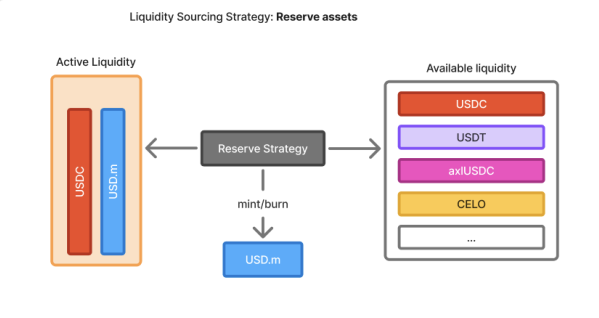
\includegraphics[width=0.6\linewidth]{figures/fpmm_3.png}
    \caption{Reserve strategy: mint\/burn at the oracle price using Reserve collateral.}
\end{figure}

\subsubsection{Mento CDP Liquidity Strategy}\label{str:cdp}
This module services \emph{synthetic} stablecoins that
are created by posting another on-chain asset as collateral inside a CDP
engine.  We illustrate the mechanics with the pair
\texttt{JPY.m}\,$\leftrightarrow$\,USD.m—JPY.m is the synthetic JPY stablecoin
and USD.m is the collateral locked in CDPs.

In Liquity~V2~\cite{liquity_v2} the Stability Pool is a
contract that holds deposits of the \emph{stablecoin} (here JPY.m) and absorbs
liquidations when troves (= CDP positions) fall below the required collateral ratio.  We extend
this design so that the Stability Pool can also act as the counterparty to
flash-swaps: it is allowed to temporarily lend JPY.m to the FPMM as long as it
receives the equivalent amount of USD.m (or vice-versa) in the same
transaction.  This small change lets one contract both maintain solvency of the
CDP system \emph{and} keep the FPMM balanced.\\

In the Mento CDP Liquidity Strategy, flash-swaps work as follows:
\begin{itemize}
  \item \textbf{Flash\hyp swap expand} – If traders have emptied the
        pool's JPY.m side, the strategy atomically 
        It (i) withdraws the missing JPY.m from the Stability Pool and (ii)
        deposits the required amount of USD.m back into the Stability Pool—
        all within a single transaction.
        The pool ends up replenished with fresh JPY.m, while the Stability Pool
        records an equal USD.m claim.
  \item \textbf{Flash\hyp swap contract} – If the pool is long JPY.m and
        short USD.m, the strategy reverses the above trade: it withdraws USD.m
        from the Stability Pool, repays JPY.m and burns the surplus.  The pool
        regains its target ratio.
\end{itemize}
\begin{figure}[ht]
    \centering
    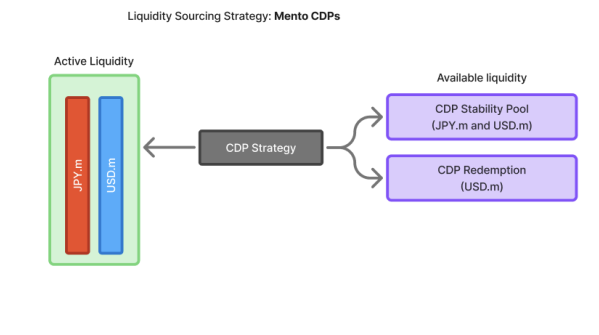
\includegraphics[width=0.6\linewidth]{figures/fpmm_1.png}
    \caption{CDP strategy: Stability Pool acts as counterparty for pool rebalances.}
\end{figure}

\subsubsection{3rd\hyp Party Provider Strategy}\label{str:external}
This Liquidity Strategy is intended for \emph{externally issued, fiat-backed}
stablecoins whose issuer wants to bootstrap on-chain liquidity without
operating a CDP or depositing collateral into the Mento Reserve.  Example pair:
\texttt{JPYx}\,$\leftrightarrow$\,USD.m where JPYx is the fiat-backed JPY
stablecoin and USD.m is the counter-asset.\\

The issuer deploys a minimal contract that
implements the flash\hyp swap interface.  Whenever the pool is short JPYx the
contract mints fresh JPYx (backed by off\hyp chain yen reserves) and withdraws
the corresponding USD.m.  When the pool is long JPYx the contract buys back and
burns the surplus with USD.m, re\hyp depositing the dollars on\hyp chain.  The
strategy logic is opaque to Mento—the only invariant enforced is that the pool
cannot lose value during the flash\hyp swap.
\begin{figure}[ht]
    \centering
    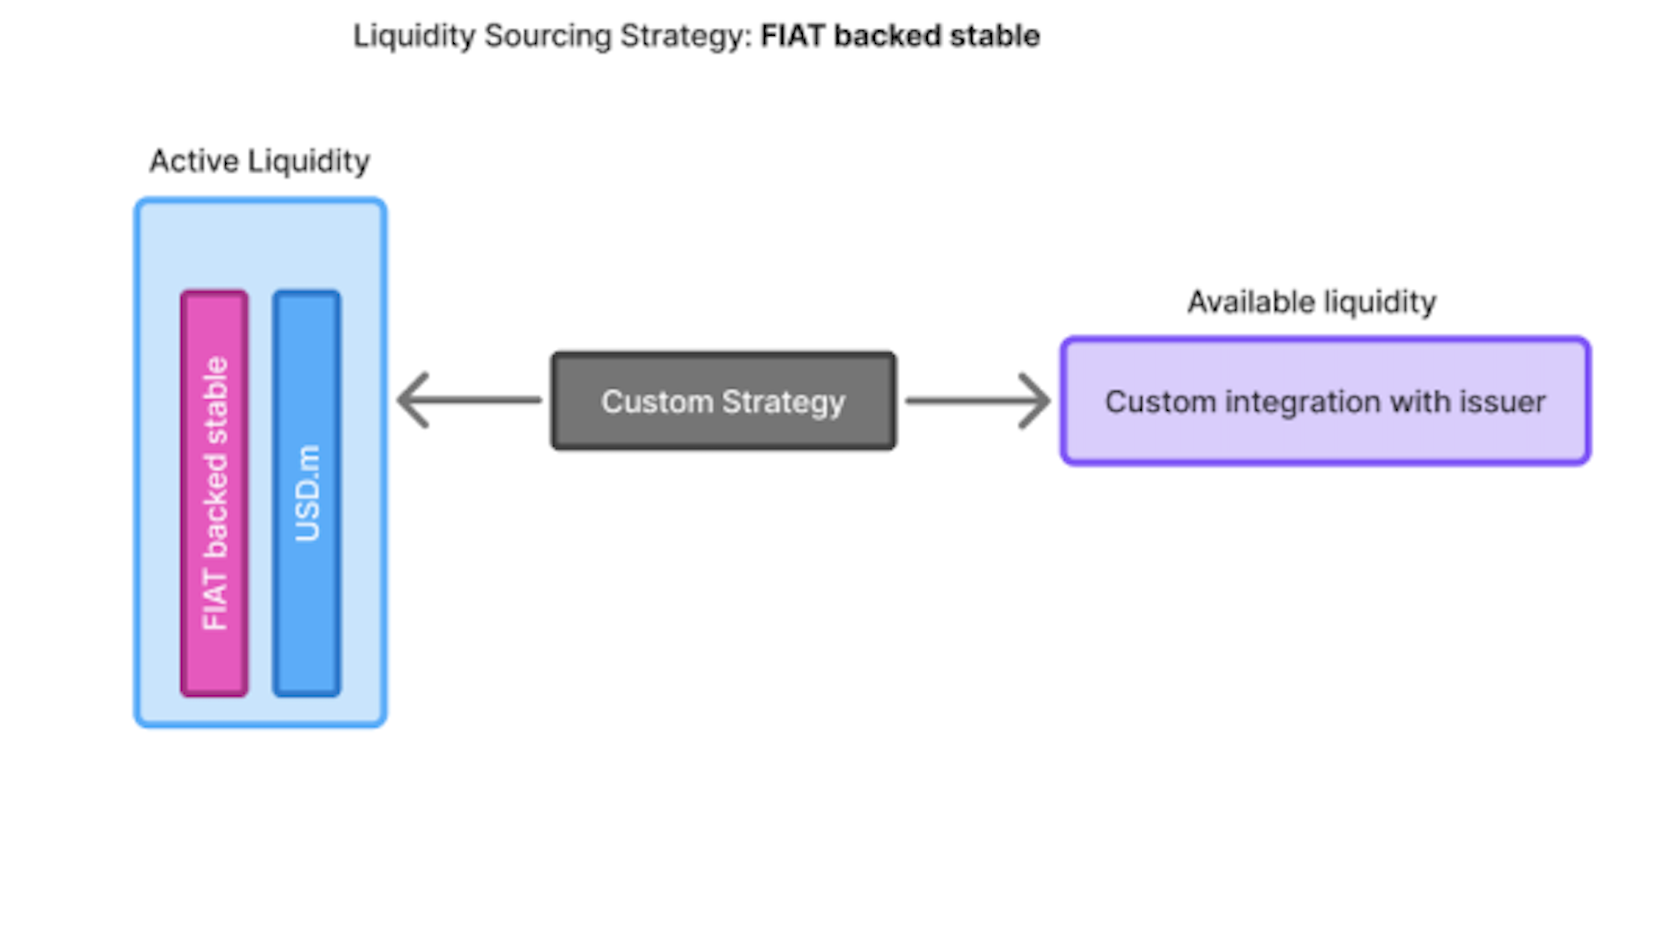
\includegraphics[width=0.6\linewidth]{figures/fpmm_2.png}
    \caption{Third\hyp party strategy: custom liquidity module keeps the pool balanced.}
\end{figure}

Together these strategies ensure FPMMs always quote deep two\hyp sided liquidity at the true
FX rate—regardless of demand imbalances, oracle downtime or market closures.

\subsubsection{Liquidity Strategies: Shared Implementation Components}\label{str:onchain}
Every concrete strategy inherits from the \verb|LiquidityStrategy| abstract base contract and must expose a single public \verb|rebalance(pool)| entry point defined in \verb|ILiquidityStrategy|.  The shared parent contract provides the following functionality:
\begin{itemize}[leftmargin=*]
  \item \textbf{Pool registry and per\hyp pool parameters}\,: Only the contract owner can add or remove pools.  For each pool the strategy stores (i) the timestamp of the last rebalance, (ii) a cooldown window that throttles successive calls, and (iii) the maximum incentive fee it is willing to pay.  These values are adjustable via admin functions \verb|setRebalanceCooldown| and \verb|setRebalanceIncentive|.
  \item \textbf{Deviation and threshold checks}\,: Prior to rebalancing the helper logic pulls the latest oracle quote as well as the pool's reserve price.  A rebalance is attempted only if the absolute deviation exceeds the pool's governance\hyp defined thresholds \verb|rebalanceThresholdAbove| or \verb|rebalanceThresholdBelow|.
  \item \textbf{Lifecycle events}\,: The strategy emits \verb|RebalanceInitiated| immediately before calling \verb|FPMM.rebalance| (thereby recording the raw token amounts and the direction of the trade) and \verb|RebalanceExecuted| after the pool confirms successful completion.
  \item \textbf{Value-preservation invariant}\,: The actual solvency check is enforced inside the pool contract itself.  After the strategy's callback has run, \verb|FPMM.rebalance| validates that (C1) the price deviation has decreased, (C2) no over\hyp shoot occurred, and (C3) the pool value did not decline by more than the allowed incentive \(\gamma\).  Should any condition fail, the entire transaction reverts, ensuring that a faulty strategy implementation cannot drain liquidity.
  \item \textbf{Extensibility hook}\,: Derived contracts override \verb|_executeRebalance|, compute the token movements specific to their liquidity source, and implement a \verb|hook| function that the pool invokes during the flash\hyp swap.
\end{itemize}


% ----------------------------------------------------------------
%  Oracle & Risk Controls (
% ----------------------------------------------------------------
\subsection{Circuit Breakers and Oracle Risk Controls}\label{sec:breaker_box}
Fixed\hyp price pools only work if the oracle they reference is
trustworthy. A stale, manipulated or wildly gapping FX feed would let
traders extract inventory at an unfair rate.
Mento therefore surrounds every FPMM with a innovative \emph{Breaker Box}\,—a
multi\hyp layer circuit\hyp breaker system that watches the oracles in real
time and, if necessary, pauses trading before capital can be drained.

\subsubsection*{Key Concepts}
\begin{description}[leftmargin=*]
  \item[Circuit Breaker] The complete safety mechanism that can throttle or
        halt trading when oracle prices behave abnormally.
  \item[Rate Feed] An individual oracle stream for a specific pair such as
        CELO\/USD or USDC\/USD.
  \item[Breaker Box] The central contract that supervises all breakers and
        switches the pool's trading mode between \textit{enabled},
        \textit{inflow\/outflow blocked}, or \textit{halted}.
  \item[Breaker] A specialised contract that monitors one rate feed and
        "trips'' once its deviation rules are violated.
  \item[Trading Mode] The set of actions currently permitted for a pool;
        bidirectional by default but automatically downgraded when a breaker
        trips.
\end{description}

\subsubsection*{Breaker Types}
\begin{itemize}[leftmargin=*]
  \item \textbf{Median\hyp Delta Breaker} – Optimised for \emph{volatile pairs}
        such as CELO\/USD. It stores the previous on\hyp chain median and trips
        when the next median deviates by more than a configurable threshold
        (typically 2–3\%). Newer versions add an EMA filter for extra
        robustness.
  \item \textbf{Value\hyp Delta Breaker} – Tailored to \emph{stable pairs} like
        cUSD\/USDC. It compares the fresh rate against a fixed reference value
        (e.g.\ USD 1.00) and trips on deviations beyond a tight band (e.g.
        0.5\%).
\end{itemize}

\subsubsection*{Lifecycle of a Breaker Event}
\begin{enumerate}[leftmargin=*]
  \item \textbf{Trigger} – A new oracle report arrives; the breaker evaluates
        the update and, if the deviation exceeds its threshold, emits
        \verb|BreakerTripped|.
  \item \textbf{Halt} – The Breaker Box instantly sets the affected pool's
        trading mode to \textit{halted}, preventing further inventory movement.
  \item \textbf{Cooldown} – Subsequent oracle reports attempt an automatic
        reset but only succeed after a per\hyp feed cooldown period (30 min for
        CELO\/USD; 1 s for USDC\/USD).
  \item \textbf{Reset} – Once price action has normalised \emph{and} the
        cooldown has elapsed, the breaker emits \verb|ResetSuccessful| and the
        pool re\hyp opens.
\end{enumerate}

\subsubsection*{Real\hyp World Breaker Events}
\begin{itemize}[leftmargin=*]
  \item \textbf{CELO\/USD (17 Aug 2023):} A 20\% market crash breached the 3\%
        Median\hyp Delta threshold. Trading paused for 30 minutes and resumed
        automatically once volatility subsided.
  \item \textbf{USDC\/USD (7 May 2023):} A brief 1.1\% USDC de\hyp peg tripped a
        Value\hyp Delta Breaker with a 0.5\% band; the breaker cooled down in
        one second and trading restarted in the same block.
\end{itemize}

These episodes demonstrate that the Breaker Box can \emph{detect},\
\emph{halt}, \emph{wait}, and \emph{resume} fully autonomously, shielding LP
capital from flash crashes and oracle manipulation.\footnote{See ``DeFi
Security: Mento Circuit Breaker in Action'', Philip, Mirror.xyz, 11 Dec 2023.}

% ---------------------------------------------------------------
%  Oracle Design & Integration
% ---------------------------------------------------------------
 FPMMs are \emph{externally priced}: instead of relying on costly, endogenous price discovery they ingest high-integrity FX quotes and trade \emph{exactly} at those rates.  This design delivers deep, low-slippage liquidity while sharply reducing arbitrage dependence.

\begin{itemize}[leftmargin=*]
  \item \textbf{Oracle providers.}  Mento natively integrates two best-in-class feeds:\cite{chainlink_docs,redstone_docs}
    \begin{itemize}[leftmargin=*]
      \item \emph{Chainlink} – the industry standard, operating large Sybil-resistant node clusters with on-chain transparency; and
      \item \emph{RedStone} – a fast, cost-efficient oracle layer that packages data off-chain and posts it on demand, enabling lower latency and cross-chain reach.
    \end{itemize}
  \item \textbf{Update logic.}  Prices are pushed on-chain whenever the reference on-chain deviates by more than a governance-set threshold (for example $\pm5$,bps).  Tighter thresholds can be configured in collaboration with the oracle partners to further reduce latency.
  \item \textbf{Pricing \& spread configuration.}  Each pool chooses a bid/ask spread that is, by default, $\approx120\%$ of the update threshold (e.g. a 12 bps spread for a 10 bps threshold). Two effects follow:
        \begin{itemize}[leftmargin=*]
          \item If the oracle has not updated yet, no trade can profitably front-run the incoming price, and
          \item users are guaranteed execution within a narrow, bounded band around the off-chain FX rate.
        \end{itemize}
\end{itemize}

The layers described next limit the \emph{worst-case loss} should an extreme price jump outrun the spread before an oracle update is mined.

% ---------------------------------------------------------------
%  Oracle Risk Management Layers
% ---------------------------------------------------------------
Because oracle integrity is mission-critical, Mento provides several defensive lines:

\begin{itemize}[leftmargin=*]
  \item \textbf{Oracle circuit breakers} – trading pauses automatically if a feed deviates beyond pre-set risk bounds or stalls for longer than an expiry window.
  \item \textbf{Time-weighted trading limits} – sliding-window caps restrict the notional that can leave a pool per block/hour, containing potential inventory drain while an oracle is impaired.
  \item \textbf{Multi-provider redundancy} – all price checks consult both Chainlink and RedStone (and any future feeds) so that a single provider outage cannot bring down pricing.
\end{itemize}

Together these mechanisms keep on-chain prices in near real-time sync with the multi-trillion-dollar FX market while protecting LP capital against manipulation or downtime.

The Mento oracles (currently Chainlink and RedStone) deliver quotes such as
\emph{EUR/USD}, \emph{JPY/USD}, or \emph{GBP/USD} into the
\verb|SortedOracles| contract.  The Breaker Box monitors those feeds against a
set of governance-defined thresholds and usage limits.  Whenever one of the
guards trips, swaps through the affected FPMM pause automatically until a
governance vote (or the passage of time) re-enables them.  In essence, the
Breaker Box turns a fragile oracle dependency into a fail-safe mechanism that
protects LP capital without compromising on 24/7 availability under normal
conditions.

Mento's circuit-breaker stack is modular: individual "breaker plugs" can be
added for new assets or risk types without touching the core contracts.  Figure
\ref{fig:circuit_breaker} illustrates the architecture.

\begin{figure}[ht]
    \centering
    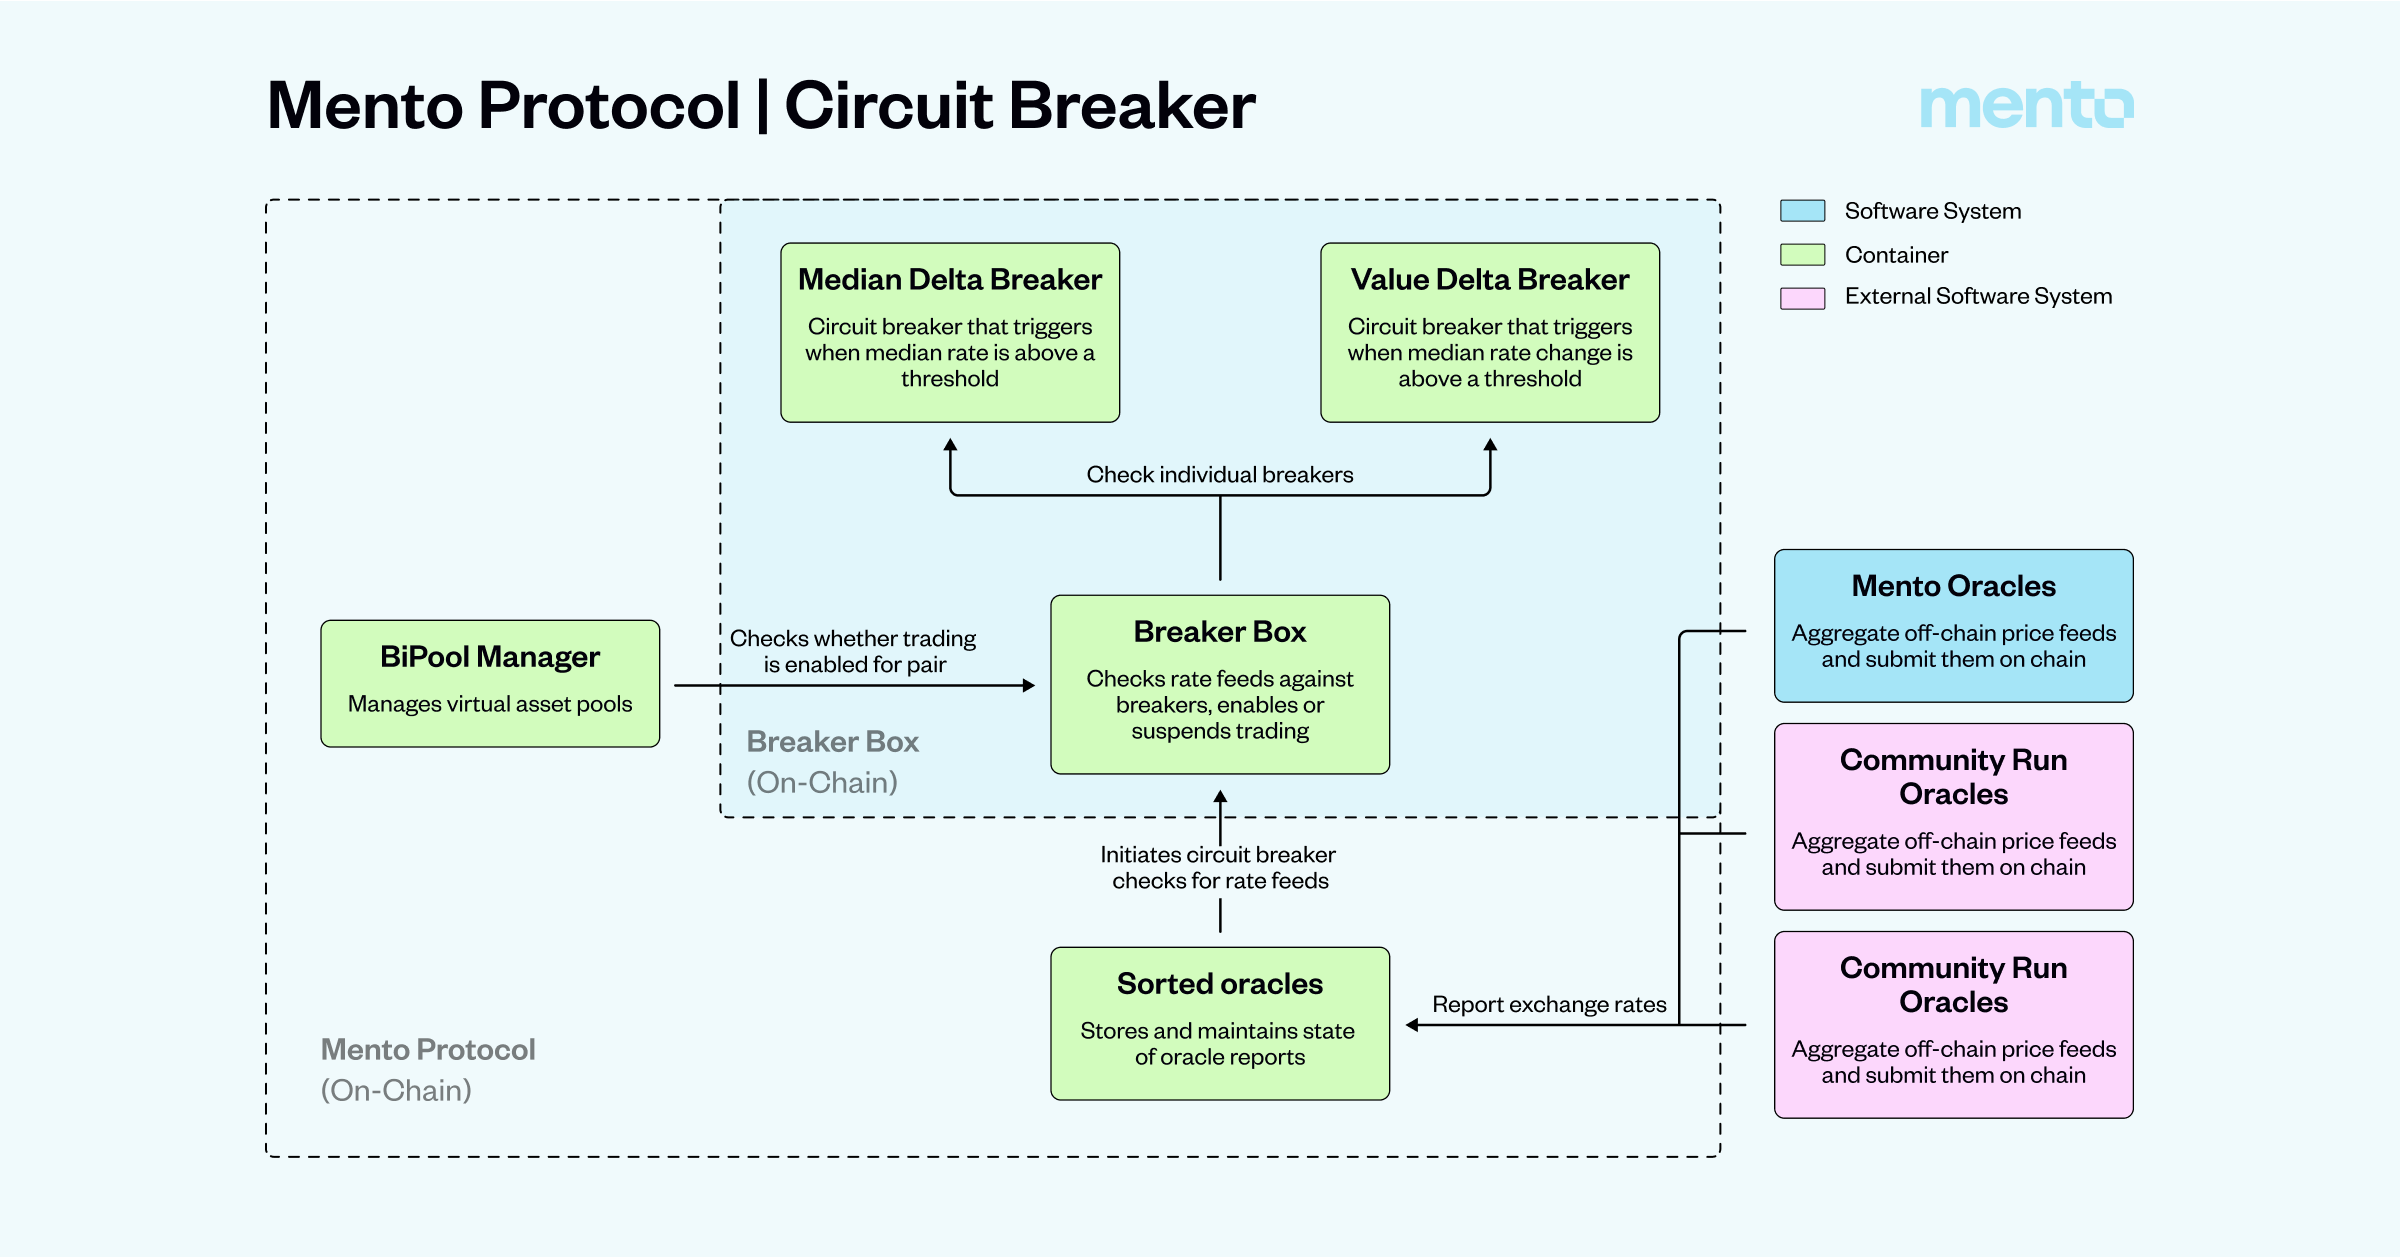
\includegraphics[width=1.0\linewidth]{figures/mento_circuit_breaker.png}
    \caption{The Mento Circuit Breaker Architecture}
    \label{fig:circuit_breaker}
\end{figure}

%  Cross-Chain Architecture
% ----------------------------------------------------------------
\subsection{Cross\hyp Chain Deployment}
FPMMs can be deployed on any EVM chain.  A hub\hyp and\hyp spoke design (Fig.~\ref{fig:cross_chain})
anchors collateral in a shared Reserve while pools on satellite chains provide native UX and
gas savings.

\begin{figure}[H]
    \centering
    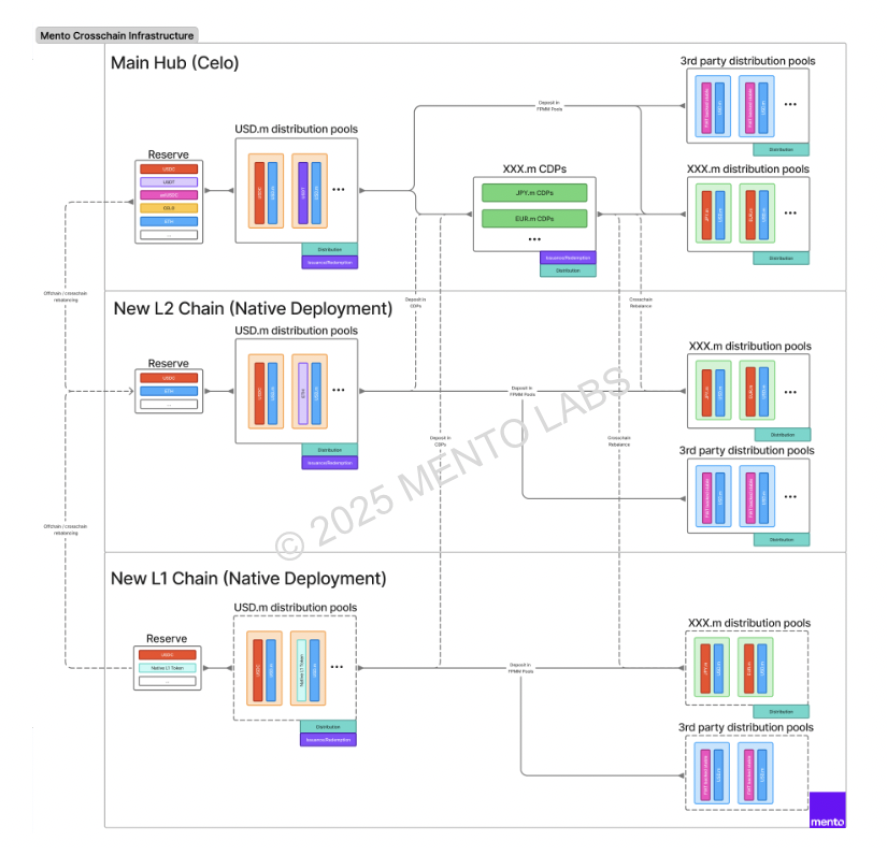
\includegraphics[width=0.75\linewidth]{figures/fpmm_4.png}
    \caption{Cross\hyp chain architecture: independent FPMM instances share collateral via a
    common Reserve.}
    \label{fig:cross_chain}
\end{figure}


\section{Mento Protocol Incentive Design}
\label{sec:incentive_structure}

Mento employs a layered incentive system that aligns every economic actor—borrowers, liquidity providers, veMENTO stakers, Stability Pool depositors and keeper bots—around three core objectives:  (i) safeguarding protocol solvency, (ii) keeping the stablecoins pegged, and (iii) creating sustainable fee income that can be shared with tokenholders. The design draws heavily on the Liquity~V2 model but adds FPMM-related incentives and governance\hyp controlled MENTO emissions.\\

\subsection{Core Incentives}
\subsubsection*{Continuous Interest and its Distribution}
\begin{itemize}
  \item \textbf{Floating interest rate}\,:  Each CDP (called ``trove'' in the Liquity V2 design Mento CDPS are based on) that mints a Mento stablecoin pays a continuously compounding interest rate $r(t)$ on its debt.
  \item \textbf{Protocol revenue stream}\,:  In addition to the interest earned on Mento Reserve assets, aggregate interest paid by all Mento stablecoin borrowers constitutes the main recurring income of the protocol (denoted $I_{\mathrm{total}}$ per block).
  \item \textbf{Split between solvency backstop and governance token}\,:  A governance parameter \texttt{SP\_YIELD\_SPLIT}\,$=\,\alpha\,\in[0,1]$ directs a fraction $\alpha I_{\mathrm{total}}$ to the Stability Pool (SP) and the remainder $(1-\alpha) I_{\mathrm{total}}$ to veMENTO stakers.  Changing $\alpha$ lets governance fine\hyp tune the risk/reward mix between backstopping liquidations and rewarding long\hyp term tokenholders.
\end{itemize}

\subsubsection*{Incentives for Stability Pool Depositors}
\begin{itemize}
  \item \textbf{Liquidation gains}\,:  When a trove falls below its collateral ratio, the SP cancels its debt and receives the collateral at a discount.
  \item \textbf{Interest share}\,:  SP depositors earn $\alpha I_{\mathrm{total}}$ pro rata, paid in the borrowed stablecoin.
  \item \textbf{Flash\hyp swap premium}\,:  When a keeper triggers a \emph{flash\hyp swap} because the FPMM has drifted off its target inventory, the strategy purchases the missing stablecoins from the SP at a slightly \emph{better} rate than the oracle price, expressed as $P_{\mathrm{oracle}}\bigl(1+\phi_{\mathrm{fs}}\bigr)$, where $\phi_{\mathrm{fs}}$ is the governance\hyp set \texttt{sp\_flashswap\_premium}.  The price premium is paid pro rata to the depositors whose stablecoins are sourced.
\end{itemize}

\subsubsection*{Rewards for veMENTO Stakers}
\begin{itemize}
  \item \textbf{Interest flow}\,:  veMENTO stakers capture $(1-\alpha) I_{\mathrm{total}}$, creating a direct link between protocol usage and token yield.
  \item \textbf{Governance rights}\,:  The same veMENTO balance determines a holder's voting weight over parameters such as \texttt{SP\_YIELD\_SPLIT}, new collateral listings or incentive emission rates.
  \item \textbf{Buyback and burn programme}\,:  Beginning immediately after the Token Generation Event (TGE), the protocol intends to plough the majority of its net revenue—including interest income, swap fees and any other cash-flows—into automated open-market repurchases of MENTO.  Purchased tokens will either be burned or deposited into the Community Treasury, creating continuous, value-accretive demand for the token and reinforcing long-term alignment between protocol usage and tokenholder upside.
\end{itemize}

\subsubsection*{Redemption Mechanics and Trove Compensation}
\begin{itemize}
  \item \textbf{Trove selection}\,:  When users redeem stablecoins for collateral, v2 targets troves with the \emph{lowest} interest rate first, effectively encouraging borrowers to keep rates competitive.
  \item \textbf{Redemption fee}\,:  The fee is paid in collateral and added \emph{directly} to the redeemed trove rather than to veMENTO stakers.  This compensates the borrower for the forced deleveraging and preserves peg stability.
\end{itemize}

\subsubsection*{FPMM Liquidity Provider Incentives}
\begin{itemize}
  \item \textbf{Spread capture}\,:  FPMM LPs quote a fixed bid/ask around the oracle price and earn the embedded spread on each user swap.
  \item \textbf{MENTO emissions via gauges}\,:  A governor\hyp controlled ``gauge'' streams a capped USD value of MENTO tokens to staked LP tokens, ensuring competitive on\hyp chain liquidity without overpaying.
  \item \textbf{Swap fee (\texttt{amm\_fee})}\,:  Every trade pays an additional micro\hyp fee that flows \emph{entirely} to LPs during normal, two\hyp sided volume.
\end{itemize}

\subsubsection*{Keeper Bots for Flash\hyp Swaps}
\begin{itemize}
\item A network of permissionless keeper bots monitors inventory drift.  When the pool breaches its tolerance band they atomically call \verb|rebalance(poolId)|, executing the flash\hyp swap.  Each successful call earns a flat, governor\hyp set MENTO bounty (denominated in USD) sized at roughly $1.5\times$ the prevailing gas cost so that maintenance remains profitable on any chain.
\end{itemize}

\subsubsection*{Balancing Incentives Across Market Regimes}
\begin{itemize}
  \item \textbf{Sideways markets}\,:  Trading volume is predominantly two\hyp sided; FPMM LPs collect both the spread and \texttt{amm\_fee}.  SP depositors earn only the baseline interest share.
  \item \textbf{Flash\hyp swap demand}\,:  One\hyp sided buying drains the pool of stablecoins.  LPs still collect the spread, \emph{but} the accumulated \texttt{amm\_fee} is forwarded to SP depositors through the flash\hyp swap premium.  The more frequently flash\hyp swaps are required, the higher the SP yield.
\end{itemize}

% ----------------------------------------------------------------
%  Actor / Position Matrix
% ----------------------------------------------------------------
\subsection{Protocol Actors and their Positions}
Fixed\hyp price markets do not impose a single "LP versus trader" dichotomy.
Instead, they let users pick \emph{where on the stack} they want to sit and what
kind of risk they are willing to absorb—be that FX exposure, liquidation risk
or pure inventory rebalancing.  The matrix below maps the directional position
and payoff profile for each archetype in a representative pool
\texttt{JPY.m}\,$\leftrightarrow$\,USD.m.  The same logic applies to any
FPMM: one asset is the \emph{stablecoin leg} (here JPY.m) and the other is the
\emph{collateral leg} (here USD.m).  A \emph{long} column marks the asset the
actor ultimately owns, while the \emph{short} column shows what they have
effectively sold or pledged.

\medskip
 
\begin{table}[ht]
    \small
    \centering
    \ra{1.3}
    \begin{tabularx}{\linewidth}{@{}l c c X X@{}}
        \toprule
        \textbf{Actor} & \textbf{Long} & \textbf{Short} & \textbf{Profits When} & \textbf{Loses When} \\ \midrule
        CDP Borrower & USD & JPY & JPY weakens vs USD & JPY strengthens vs USD \\ 
        Stability Pool Depositor & JPY.m & none & JPY strengthens, fees through liquidations or block swaps & JPY weakens \\
        Mento Reserve & Reserve assets & Circulating USD.m & Collateral stays pegged & Collateral de\hyp pegs \\
        3rd\hyp Party Issuer & Withdrawn collateral & Their token in pool & Collateral outperforms token & Must buy back above par \\
        LP Provider & FPMM inventory & \textemdash & Earn swap fees & Oracle failure or price gap \\
        Spot Trader & Purchased token & Sold token & Market appreciation & Market depreciation \\ \bottomrule
    \end{tabularx}
    \caption{Indicative exposures for key actors interacting with an FPMM in the example of a JPY stablecoin, backed by USD collateral.}
    \label{tab:fpmm_positions}
\end{table}

Practically this means:
\begin{itemize}[leftmargin=*]
  \item A \textbf{CDP borrower} expresses a leveraged belief that the
        stablecoin will \emph{depreciate} against the collateral and earns that
        upside in the form of cheap synthetic liquidity.
  \item A \textbf{Stability Pool depositor} earns liquidation yield and flash\hyp
        swap fees for providing the inventory that offsets the borrower—an
        attractive play for yield seekers happy to be long the stablecoin.
  \item The \textbf{Mento Reserve} and \textbf{3rd\hyp party issuers} capture
        basis spread by financing the system with low\hyp risk collateral or
        RWAs.
  \item \textbf{Liquidity providers} bet on sideways markets in which they harvest swap
        fees as compensations for providing liquidity.
  \item \textbf{Spot traders} leverage the infrastructure without ever thinking
        about these mechanics; they just receive a guaranteed rate.
\end{itemize}
This flexibility is a core strength of the FPMM design: every risk has a
counterparty, and every counterparty is compensated transparently on\hyp chain.


\section{Additional Components of the Mento Platform}\label{sec:additional_components}
This section provides an overview over the building blocks that, in addition to the DEX infrastructure provided by the Mento FPMMs, form the Mento Platform. Section \ref{sec:stables} dives into the properties and uses-cases for the wide range of stablecoins that are already live on Mento whereas \ref{sec:gov_token} goes into detail on the MENTO governance token and its role and utility in the Mento protocol. 

\subsection{Mento Stable Assets}\label{sec:stables}
All Mento stablecoins are \emph{distributed and traded primarily via FPMMs}.  The provision of useful stable assets is the ultimate goal of the Mento Platform, addressing the volatility common in traditional cryptocurrencies and offering a dependable means for a wide array of financial use-cases. The properties and uses-cases of Mento stable assets are shaped by several innovative features and a range of integrations and tooling.

\begin{itemize}
    \item Paying for Gas Fees with Stablecoins: A tremendously helpful feature of Mento stablecoins is their use as gas currency on the Celo blockchain. This allows users to conduct transactions using stablecoins directly, eliminating the need for holding multiple assets for gas payments. Notably, the transaction fees on Celo are extremely low, significantly reducing the cost barrier for users. This combination of properties makes Mento stablecoins ideal for end-user focused use cases.
    
    \item Trading and FX Capabilities: Mento stablecoins offer efficient trading mechanisms among themselves, enabling various FX-related use cases. This capability facilitates seamless currency exchange and effective risk management strategies, broadening the platform's utility for users engaged in multi-currency operations.
    
    \item Decentralized Governance and Control: Unlike centralized stablecoins such as USDC (Circle) and USDT (Tether), which are under the control of specific profit-oriented entities, Mento stablecoins benefit from a decentralized governance structure provided by the Mento Platform. This setup ensures that decisions regarding the stablecoins, including their issuance (for example issuance and redemption fees), management, and operational protocols, are made collectively by the community and stakeholders through a transparent and democratic process. This contrasts sharply with centralized stablecoins, where decisions are made behind closed doors and can be influenced by the controlling company's interests. The decentralized nature of Mento stablecoins aims to enhance trust, reduce single points of failure, and ensure a broader, long-term alignment with the users' and community's interests.
    
    \item Customization: Mento empowers users to create and manage their own stablecoins, designed to meet specific requirements and use cases. Mento provides options for creating both, collateral-debt-position-based and reserve-model-based stablecoins. This flexibility allows issuers to select the model that aligns with their risk management preferences and the economic dynamics of their target use case. This level of customization and flexibility supports a wide range of applications, from local community currencies to tailored settlement currencies.
    
    \item FiatConnect API Integration: The integration with the FiatConnect API standard significantly enhances the interoperability of Mento stable assets with various fiat on- and off-ramps. This ensures smooth transitions between fiat and digital assets, improving the accessibility for users to enter and exit the digital asset ecosystem.
    
    \item Integration with Transaction Routers: The integration of Mento stable assets into transaction routers, such as the Squid router, streamlines the process of moving these assets across different blockchain networks. This integration boosts liquidity and accessibility, making stablecoins more user-friendly and versatile.
    
    \item Integration in Popular Wallets: Mento stablecoins are integrated into popular end-user facing wallets, including Opera's MiniPay and Valora. Such integrations significantly enhance the accessibility and usability of Mento stablecoins for a broad user base, allowing for easy storage, management, and transfer. The presence of Mento stablecoins in these wallets demonstrates that its digital assets are convenient to use for everyday transactions, further bridging the gap between traditional financial systems and Web3 technology.
\end{itemize}

The following sections provide more detail about the Mento Platform components that help achieve the above properties and ultimately make Mento stablecoins useful in the real world. For even more technical details, please visit Mento on GitHub \cite{mento_github}.

\subsection{ MENTO Governance Token}\label{sec:gov_token}

\subsubsection{Governance Architecture}
\begin{figure}[ht]
    \centering
    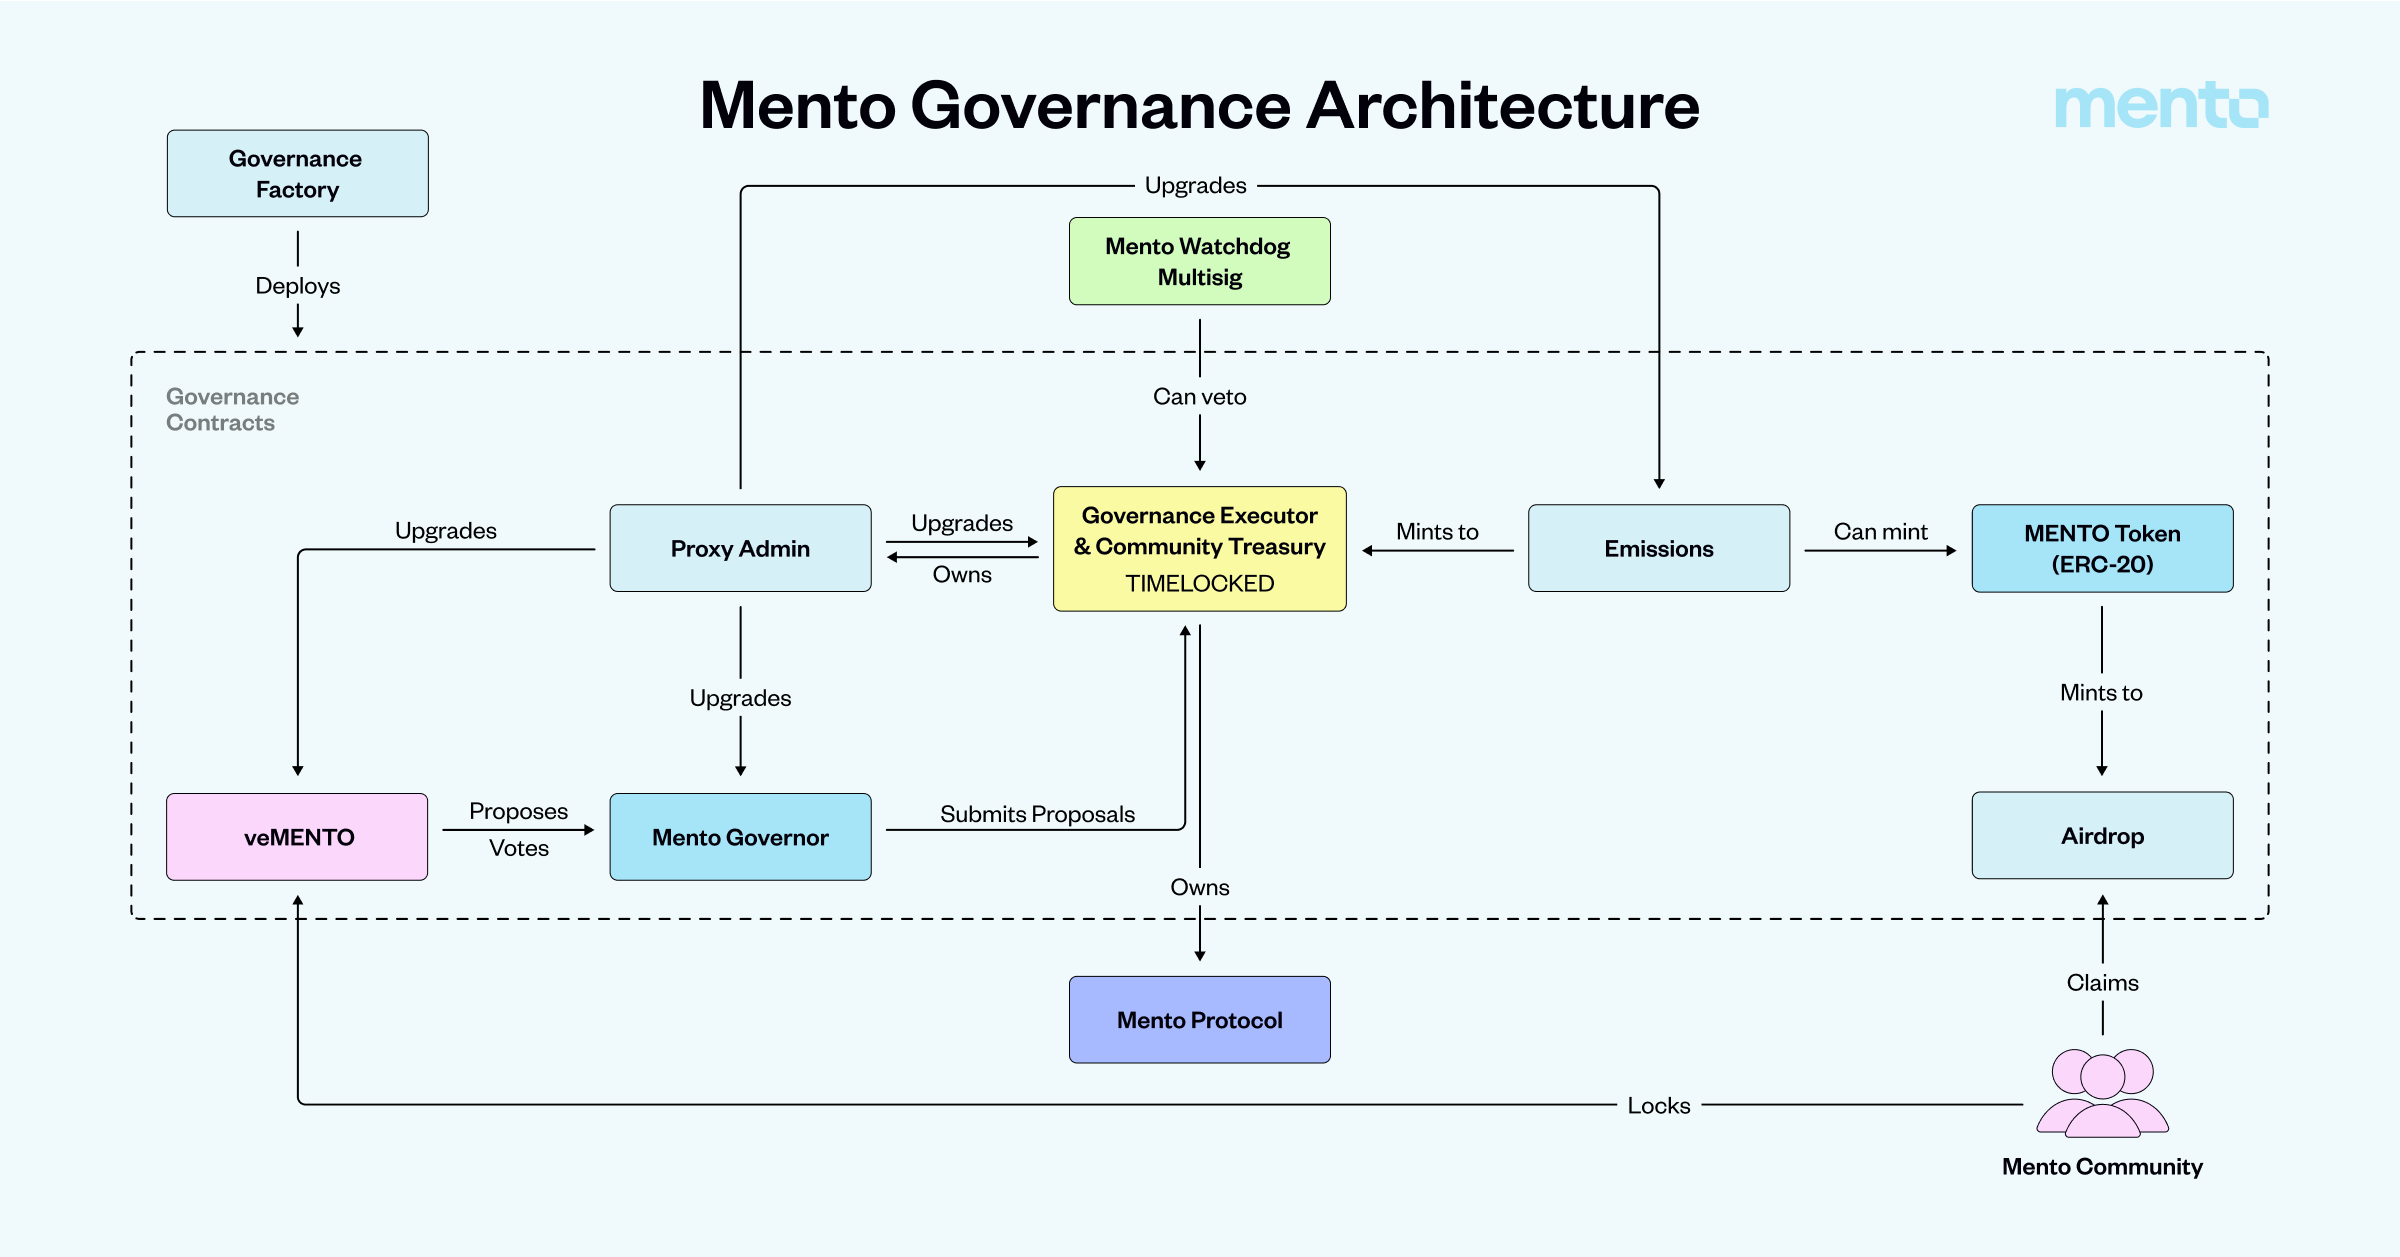
\includegraphics[width=1\linewidth]{figures/mento_governance.png}
    \caption{This figure illustrates the architecture of Mento Governance.}
    \label{fig:mento_governance}
\end{figure}
In addition to the MENTO token, the Mento Protocol introduces veMENTO (vote-escrowed MENTO), a locked version of the token that empowers holders to actively participate in the governance process. The veMENTO concept draws inspiration from the veModel, an on-chain governance framework pioneered by Curve Finance~\cite{curve_vemodel} and embraced by numerous protocols.

veMENTO holders demonstrate a long-term commitment to the protocol by locking their tokens for varying durations, ranging from one week to four years. This mechanism incentivizes sustained engagement and rewards individuals who contribute to the protocol's long-term success. Through veMENTO, holders accrue enhanced voting power commensurate with the duration of their lock-up period, amplifying their influence in shaping governance decisions and fostering a vibrant and resilient ecosystem.

Key smart contract components of Mento governance are illustrated in Figure \ref{fig:mento_governance} and include:
\begin{itemize}
    \item ERC-20 Smart Contract: The MENTO token functions as an ERC-20 standard token, facilitating seamless integration with decentralized applications and exchanges.
    \item Voting Escrow: A staking contract allows users to lock MENTO tokens in exchange for veMENTO tokens which represent governance rights, encouraging active participation and rewarding long-term commitment.
    \item Governor Contracts: On-chain governance contracts oversee smart contracts, treasury management, reserve allocation, and protocol adjustments in a decentralized manner.
    \item Emission Contract: Controls the issuance of MENTO tokens to the treasury, regulating protocol spending and ensuring sustainable growth.
    \item Community Treasury: Receives emissions from MENTO tokens, enabling governance to allocate resources efficiently and support platform initiatives.
    \item Watchdog Multisig: In general terms, a "watchdog" refers to an individual or group that monitors the activities of another entity (such as an individual, corporation, non-profit group, DAO, community, or governmental organization) on behalf of the public to ensure that the entity behaves according to its set purpose and does not act illegally or unethically. In the case of the Mento Protocol, in particular, a watchdog means a group of individuals who will oversee the protocol's governance process, making sure that the technical part of the governance proposals (execution code) exactly matches what's written in the proposal itself. Initially, it is a 3 out of 9 SAFE multi-signature wallet (multisig) with a special right to veto (meaning to cancel the execution of) any governance proposal within 48 hours after it passes.
\end{itemize}

\subsubsection{Tokenomics and Distribution}\label{sec:token_distribution}
At the genesis block (the block at which the MENTO token and governance are deployed), the MENTO token will be non-transferable. Holders can claim their allocation, locked as veMENTO, and participate in governance, but not transfer tokens. At some point in the future, when certain milestones decided by the community have been reached, the transferability of the token will be enabled. At that point in time, it should be possible to sell/buy the token on a secondary market and freely transfer it. The enabling of transferability is subject to on-chain governance.

The allocation plan for the MENTO token was developed to embody fairness, foster community engagement, and ensure the ecosystem's sustainability. The initial token supply allocation contains a notable 45\% designated to the Mento Community Treasury. This allocation is pivotal for providing sufficient resources for the platform's continuous development, the advancement of community-centric initiatives, and the broad growth of the ecosystem.

The MENTO token will have a maximum total supply of 1,000,000,000 (one billion) tokens (also referred to as fully diluted supply going forward). Figure \ref{fig:mento_distribution} provides a high-level overview over the initial distribution. More detail on each individual distribution is provided thereafter.

\begin{figure}[ht]
    \centering
    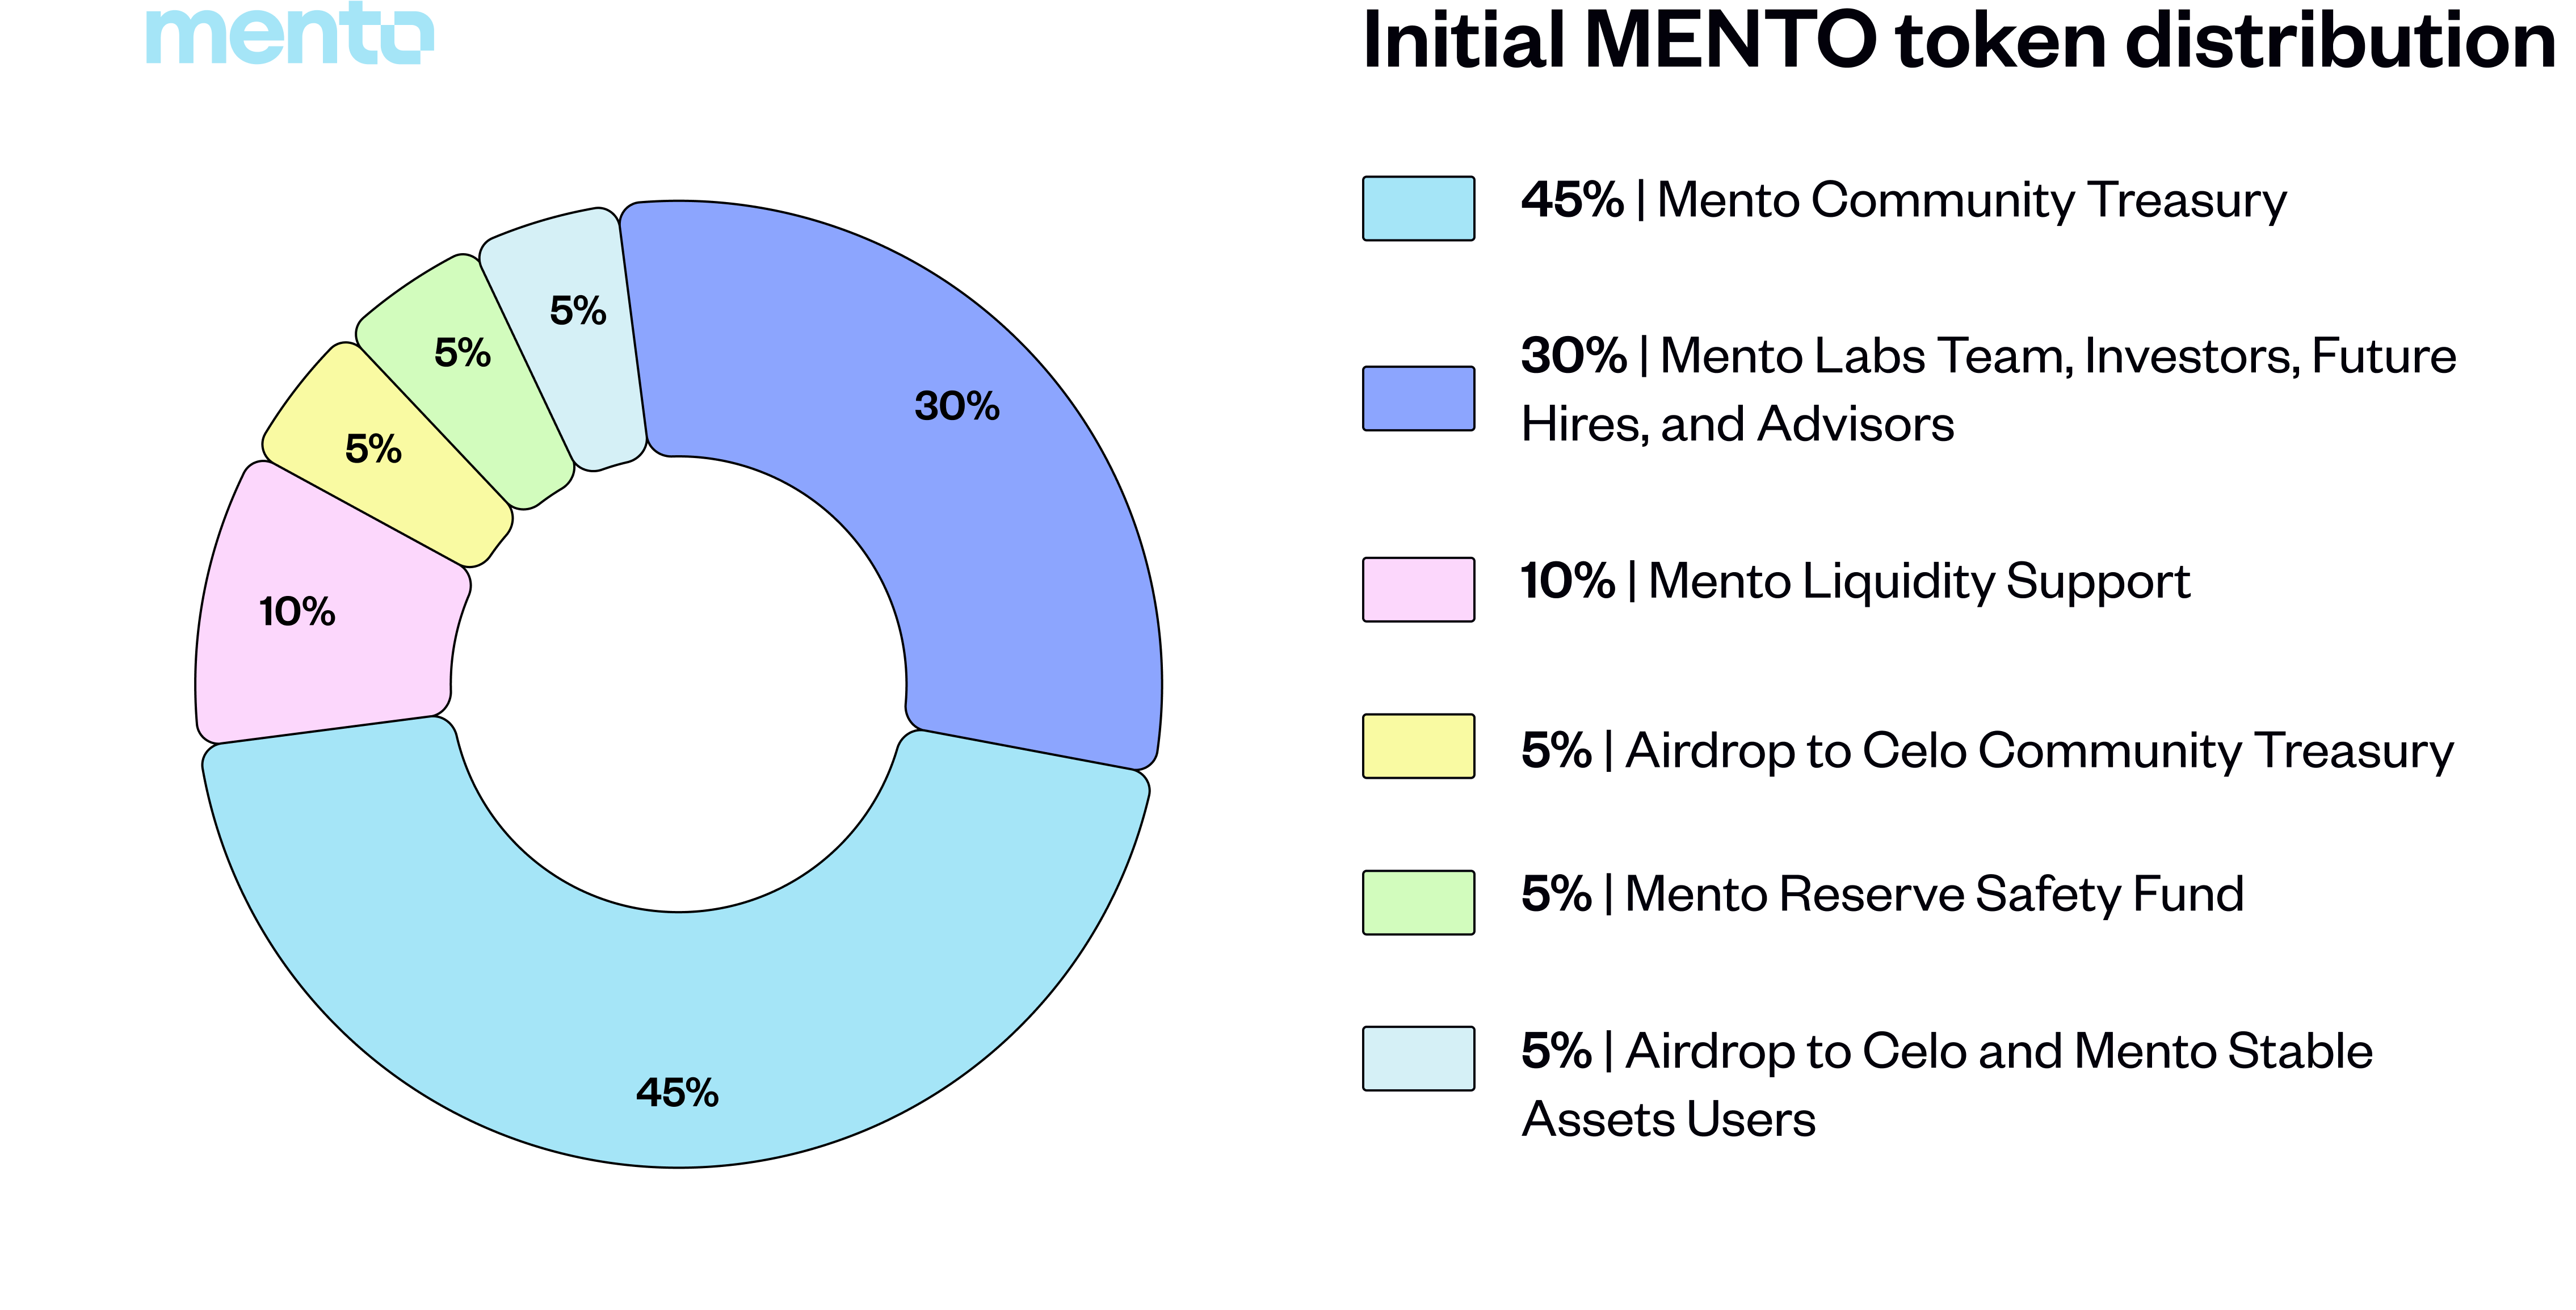
\includegraphics[width=1\linewidth]{figures/mento_distributions.png}
    \caption{MENTO token allocation.}
    \label{fig:mento_distribution}
\end{figure}

\subsubsection*{Mento Community Treasury}
\begin{itemize}
    \item Purpose: The Mento community can spend tokens from the treasury to foster the platform's development. The tokens can be spent on grants, liquidity incentivization programs, etc. The decision to spend tokens from the Treasury is always subject to governance.
    \item Distribution: 450M tokens (45\% of fully diluted supply) with 50M available at genesis block. The tokens will be emitted to the Treasury via exponential decay with a half-life of 10 years. This approach aims to manage the introduction of new tokens into the market gradually and provides an upper bound on spending for the Mento Community Treasury. The emission schedule over time is visualized in Figure \ref{fig:mento_emissions}.
    \item Voting rights: No.
\end{itemize}
\begin{figure}[ht]
    \centering
    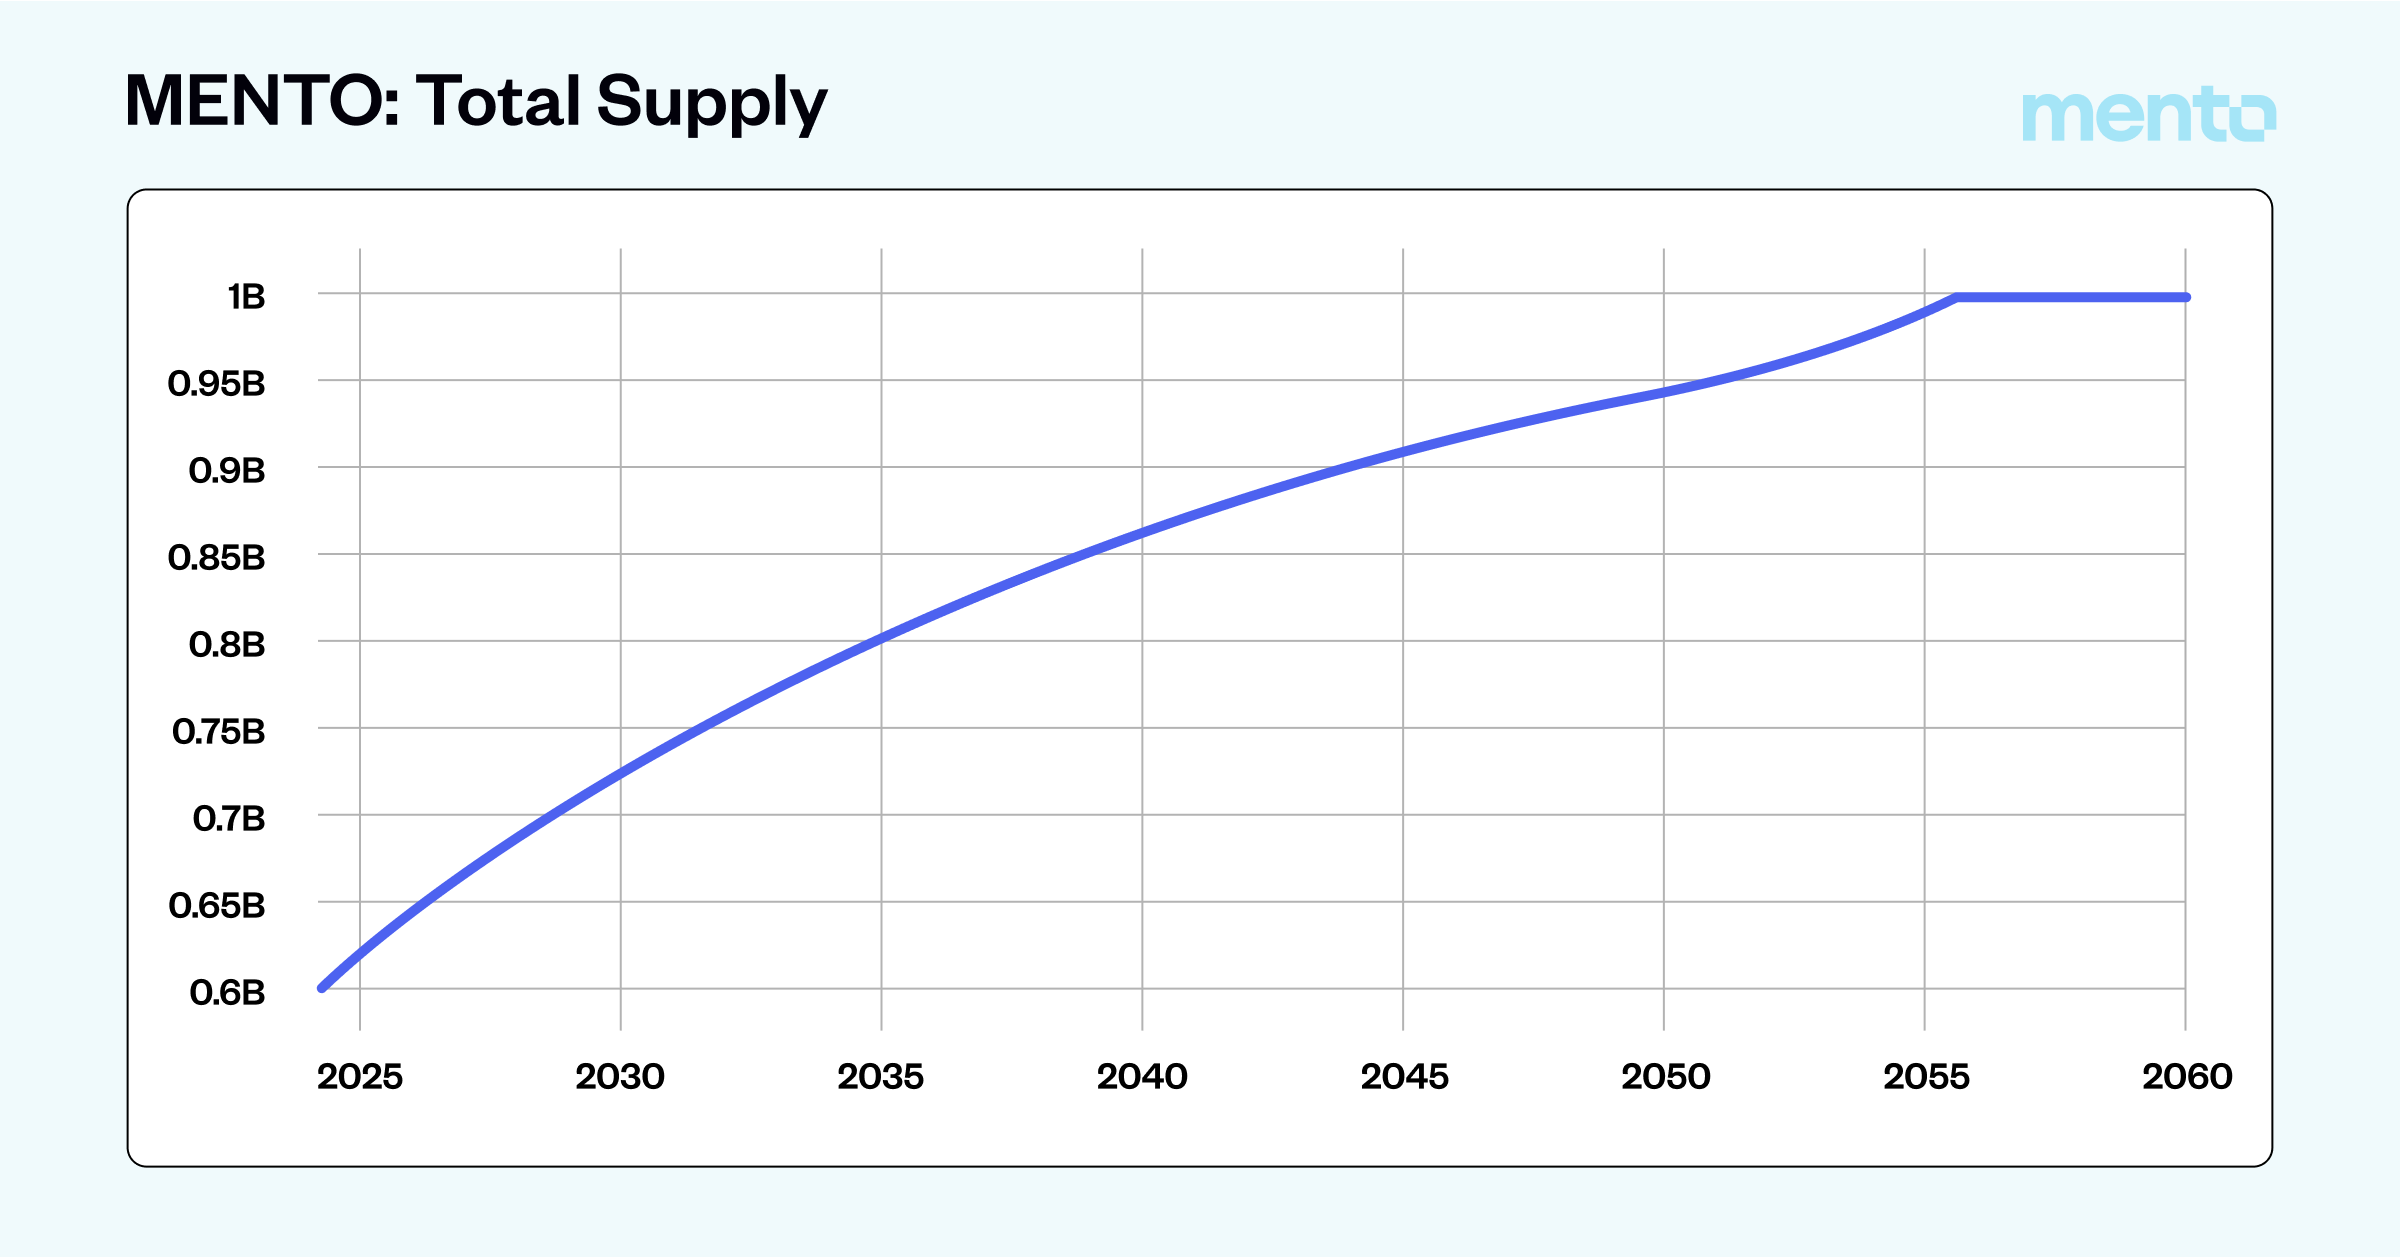
\includegraphics[width=1\linewidth]{figures/mento_emissions.png}
    \caption{MENTO token emissions over time.}
    \label{fig:mento_emissions}
\end{figure}


\subsubsection*{Mento Labs Team, Contributors, Supporters, Future Hires, Advisors}
\begin{itemize}
    \item Purpose: Reward core contributors, supporters, and advisors. Get the best talent to contribute to the protocol in the future.
    \item Distribution: 300M tokens (30\% of fully diluted supply). Existing Mento Labs employees\footnote{For information on Mento Labs, see \cite{mento_labs_website}.}, supporters, and advisors will receive their MENTO tokens split into two parts:
    \begin{itemize}
        \item veMENTO portion (25\% of the allocation):
        To seed voting power to the team and supporters, 25\% of the allocation will be distributed as veMENTO locked for 1 year starting at the token distribution event. The allocation will allow team members to vote from day one using delegation. However, the beneficiary will only get full control of the lock after their cliff period has passed.
        \item MENTO portion (75\% of the allocation): 75\% as MENTO with 1 year delay and 3 years linear vesting starting at the token distribution event via Hedgey token vesting platform. 
    \end{itemize}
    \item Voting rights: Yes, with the veMENTO portion.
\end{itemize}

\subsubsection*{Airdrop to CELO holders and Mento Stable Assets users}
\begin{itemize}
    \item Purpose: Reward existing community members and users for their past contributions to the development and usage of Mento stable assets and the Celo ecosystem overall. 
    \item Distribution: 50M tokens (5\% of fully diluted supply). Owners of eligible addresses can claim their allocation, which they will receive as a veMENTO locked for 2 years with linear unlock. Eligibility criteria apply.
    \item Voting rights: Yes.
\end{itemize}


\subsubsection*{Airdrop to Celo Community Treasury}
\begin{itemize}
    \item Purpose: Long-term incentive alignment between the Celo and Mento communities.
    \item Distribution: 50M (5\% of fully diluted supply) with a 2-year delay followed by a 6-year linear vesting period via the \href{https://hedgey.finance/}{Hedgey} token vesting platform.
    \item Voting rights: No.
\end{itemize}

\subsubsection*{Mento Reserve Safety Fund}
\begin{itemize}
    \item Purpose: An allocation to the Mento Reserve, which will be used as stablecoin collateral in the worst-case scenario of a loss-of-value in primary collateral (USDC, USDT, DAI, …) through credit default events, hacks, etc. 
    \item Distribution: 50M (5\% of fully diluted supply)
    \item Voting rights: No.
\end{itemize}

\section{Roadmap and Future Developments}
\label{sec:roadmap}

The Mento Platform's development path is structured around clear, actionable objectives aimed at broadening its financial ecosystem. Central to this expansion are the introduction of the MENTO token and the establishment of a decentralized governance structure.

\begin{itemize}
    \item \textbf{Governance Transition:}
    The Mento Governance was activated on (July 2025) and the MENTO token was previously distributed according to the allocations described in Section \ref{sec:token_distribution}. This new structure now empowers the community to propose, debate, and implement changes directly through a democratic voting process. Initial governance actions will focus on community-led development and innovation. 

    \item \textbf{Token Generation Event:}
    The Token Generation Event (TGE), which will activate the transferability of the MENTO token, is planned for Q3/2025. MENTO will serve as the cornerstone of the platform's governance model, enabling token holders to vote on key proposals and influence the platform's direction. The token transferability is a critical step towards decentralizing decision-making processes and aligning the platform's development with the community's needs and values. It will also allow for incentivizing certain behavior on the platform and directing and sharing platform revenue.
    
    \item \textbf{Integration and Partnership Enhancements:}
    Beyond internal developments, the roadmap includes strategic partnerships aimed at enhancing platform interoperability and user access. These collaborations will extend the reach of Mento's stablecoins and the MENTO token across various blockchains, wallets, exchanges, and DeFi platforms, ensuring seamless integration into the broader digital asset ecosystem. 
    
    \item \textbf{FX Trading and Hedging Functionalities:}
    Following the token launch and governance initiation, targeted improvements protocol will introduce advanced functionalities for FX trading and hedging. These features are designed to support both individuals and businesses in managing exposure to currency volatility, further cementing Mento's role in facilitating global commerce and finance.

\end{itemize}

Each component of the roadmap is crafted to enhance the Mento Platform's offerings, governance, and integration within the global financial landscape. By focusing on these key areas, Mento aims to provide a more inclusive, efficient, and user-driven digital asset platform.

\section{Conclusion}
\label{sec:conclusion}
This paper has presented a comprehensive specification of the Mento Protocol and its central building block—the \emph{Fixed-Price Market Maker (FPMM)}. By anchoring on-chain liquidity to a multi-source oracle and enforcing deterministic flash-swap rebalancing guarded by layered circuit breakers, FPMMs achieve foreign-exchange execution that mirrors off-chain reference rates while maintaining pool solvency.

Three complementary liquidity strategies—Reserve, CDP, and Third-Party—illustrate how heterogeneous collateral sources can interface with the same flash-swap invariant. The quantitative analysis established that (i) user swaps are always value-accretive and (ii) any rebalance profit is bounded by a governance-set incentive cap, thereby limiting adverse inventory loss and oracle-front-running risk.

Beyond pool mechanics, the whitepaper detailed an incentive architecture that aligns Stability Pool depositors, veMENTO stakers, FPMM keeper bots, and FPMM liquidity providers. The \texttt{MENTO} governance token, distributed according to Section~\ref{sec:token_distribution}, steers parameter updates, collateral listings, and emission gauges through on-chain voting. Combined with a circuit-breaker stack and time-weighted trading limits, the protocol offers a robust defence against oracle failure, extreme market moves, and governance capture.

The development roadmap prioritises (i) activation of transferable \texttt{MENTO} and full community governance, (ii) cross-chain deployments that connect satellite pools to a shared Reserve hub, and (iii) extension of the FPMM spot trading design into derivative markets. Each milestone will be executed transparently and subjected to open economic and security reviews.

By unifying deterministic pricing, programmatic liquidity management, and decentralised governance, Mento aspires to furnish a public, 24/7 FX layer that matches the pricing efficiency of traditional desks while achieving sub-second finality and remaining permissionless and composable. The authors invite researchers, auditors, and practitioners to scrutinise and extend the open-sourced contracts and formal models presented herein.



\begin{appendices}

\section{Compliance with MiCAR Title II Regulations}
\label{sec:micar}
The Markets in Crypto-Assets Regulation (MiCAR), specifically Title II, sets forth guidelines for \textit{crypto-assets other than asset-referenced tokens or e-money tokens}. Accordingly, this section focuses on the Mento token as opposed to Mento stablecoins, which are subject to different regulatory criteria.

Article 6 of Title II within MiCAR details the required content and format for a crypto-asset white paper. This part of our white paper is designed to meet those requirements, aiming for compliance with the regulatory framework outlined by MiCAR. The structure of this section and the information it includes are intended to closely follow Article 6's guidelines and structure. This aims to ensure that stakeholders, including potential investors and others interested in the Mento ecosystem, are well-informed about the Mento token's compliance status, associated risks, and its operational setup, supporting well-informed decisions based on a thorough understanding of regulatory expectations and asset specifics.

\subsection{Article 6, Paragraph (1): Required Information}
The information presented in the following subsections is required to be contained in a compliant whitepaper, see MiCAR, Title II, Article 6, Paragraph (1) below:

\begin{quote}
(1) A crypto-asset white paper shall contain information about (a) the offeror (b) the person seeking admission to trading, (c) the operator of the trading platform, (d) the crypto-asset project, (e) information about the offer to the public of the crypto-asset or its admission to trading; (f) information about the crypto-asset; (g) information on the rights and obligations attached to the crypto-asset; (h) information on the underlying technology; (i) information on the risks; (j) information on the principal adverse impacts on the climate and other environment-related adverse impacts of the consensus mechanism used to issue the crypto-asset.
\end{quote}

\subsubsection{The Offeror}
\begin{itemize}
    \item Entity Name: [To be provided]
    \item Registered Office: [To be provided]
    \item Contact Information: [To be provided]
    \item Legal Status and Structure: [To be provided]
\end{itemize}

\subsubsection{Person Seeking Admission to Trading}
\begin{itemize}
    \item Entity Name and Role in Project: [To be provided]
    \item Contact Information and Legal Details: [To be provided]
\end{itemize}

\subsubsection{Operator of the Trading Platform}

\textbf{Mento Labs GmbH} acts as the operator of the trading platform within the Mento ecosystem, focusing on technological development and improvements to the Mento protocol.

\begin{itemize}
    \item \textbf{Registered Office:} Lohmühlenstraße 65, 12435 Berlin, Germany
    \item \textbf{Contact Information:} Email: \texttt{contact@mentolabs.xyz} | Website: \url{https://mentolabs.xyz}
    \item \textbf{Legal Status:} GmbH (limited liability company)
    \item \textbf{Managing Directors (Geschäftsführer):} Dr. Markus Franke
    \item \textbf{Commercial Register:} Amtsgericht Charlottenburg HRB 247880B
    \item \textbf{VAT-ID:} DE359437810
\end{itemize}
\begin{itemize}
    \item \textbf{Name:} Dr. Markus Franke
    \item \textbf{Address:} Lohmühlenstr. 65, 12435 Berlin, Germany
\end{itemize}

\subsubsection{The Crypto-Asset Project}
The Mento project is an initiative aimed at leveraging web3 technology to enhance financial inclusivity and sustainability across the globe. At the core of the Mento ecosystem is the development and deployment of stablecoins that prioritize ease of use, security, and accessibility. 

\begin{itemize}
    \item \textbf{Overview and Objectives:} Mento's mission is to deliver a permissionless, 24/7 foreign-exchange layer that mirrors off-chain FX rates on-chain.  It couples oracle-anchored \emph{Fixed-Price Market Makers (FPMMs)} with modular liquidity strategies so that anyone can issue, distribute and trade local-currency stablecoins at deterministic prices.  The ultimate goal is to remove the frictions of traditional FX rails and make programmable money—priced in the currencies people actually use—available to every smartphone user.
    
    \item \textbf{Current Development Stage:} As of July 2025 the FPMM v3 contracts are in the process of being deployed on Celo main-net.  Multi-source oracle feeds (Chainlink + RedStone) and the Breaker-Box circuit-breaker are fully operational.  Community governance has been activated, and the non-transferable \texttt{MENTO} token has been distributed according to the allocation plan in Section~\ref{sec:token_distribution}.  Security audits on most components are complete, and cross-chain deployment tooling is in internal test-stage.
    
    \item \textbf{Roadmap:} Moving forward, the Mento team is focused on:
    \begin{enumerate}
        \item \textbf{Governance transition}: MENTO governance went fully live in July~2025; proposals now decide parameter tuning and new initiatives.
        \item \textbf{Token Generation Event (TGE)}: Transferability of the MENTO token is scheduled for Q3~2025, unlocking emission gauges and secondary trading.
        \item \textbf{Integration and partnerships}: Ongoing collaborations will bring Mento stablecoins and MENTO to additional chains, wallets, and DeFi venues.
        \item \textbf{FX trading and hedging extensions}: Post-TGE upgrades will add advanced FX trading and on-chain hedging features.
    \end{enumerate}
\end{itemize}

The Mento community is committed to transparency, open-source development, and community-driven governance. By collaborating with developers, users, and stakeholders across the blockchain ecosystem, Mento aims to continuously innovate and adapt to the evolving landscape of digital finance, driving greater financial empowerment and inclusion worldwide.

\subsubsection{Offer to the Public or Admission to Trading}
\begin{itemize}
    \item Terms, Conditions, and Procedures of the Offer - [To be provided]
    \item Information on Trading Platforms and Admission - [To be provided]
\end{itemize}

\subsubsection{Information About the Crypto-Asset}
\begin{itemize}
    \item \textbf{Classification and Types of Mento Crypto-Assets}\\
    The Mento Token (MENTO) acts as the governance and utility token of the Mento Protocol and is distinct from Mento Stablecoins. It enables holders to participate in the governance process, influencing the Mento ecosystem's development and strategic direction.

    \item \textbf{Technology and Infrastructure Details}\\
    The MENTO token operates on the Celo blockchain, utilizing advanced smart contract architecture for secure and efficient governance actions, token distribution, and seamless integration with DeFi platforms. This framework supports decentralized governance and enhances interoperability across the blockchain ecosystem.

    \item \textbf{Functional Use Cases within the Ecosystem}\\
    MENTO tokens are instrumental in enabling:
    \begin{itemize}
        \item \textit{Governance Participation:} Holders can propose and vote on changes, driving the ecosystem's evolution in alignment with community interests.
        \item \textit{Incentive Mechanisms:} Influencing incentive structures within the ecosystem to encourage active participation and contribution.
        \item \textit{Ecosystem Development and Funding:} Facilitating ecosystem growth through strategic project funding and partnership support.
        \item \textit{Stakeholder Engagement:} Fostering a deep level of involvement from all ecosystem participants, aligning their interests with the ecosystem's success.
    \end{itemize}
\end{itemize}


\subsubsection{Rights and Obligations}
This section details the rights associated with the MENTO Tokens and the encouraged responsibilities of the holders within the Mento ecosystem, ensuring clarity on the governance participation and the potential of revenue sharing based on future governance decisions.

\begin{itemize}
    \item \textbf{Rights Attached to the Crypto-Assets}
    \begin{itemize}
        \item \textit{Governance Participation:} MENTO Token holders are welcomed to partake in the governance processes of the Mento ecosystem. This includes the ability to propose, vote, and influence the ecosystem's strategic directions and priorities, though participation is voluntary and at the holder's discretion.
        
        \item \textit{Input on Ecosystem Development:} Token holders are encouraged to offer suggestions for ecosystem improvements, including new features and optimizations, contributing to the ecosystem's evolution in a collaborative manner.
        
        \item \textit{Potential Revenue Sharing:} The possibility of platform revenue sharing exists, subject to future governance decisions. Token holders may have the opportunity to participate in the ecosystem's success through mechanisms that will be defined and approved by the community governance processes.
        
        \item \textit{Access to Services:} Holding tokens may provide opportunities for access to certain services within the ecosystem, such as early access to features or preferential terms, acknowledging the active role of token holders in the ecosystem's development.
    \end{itemize}
    
    \item \textbf{Holder Obligations}
    \begin{itemize}
        \item \textit{Engagement in Governance:} Token holders are encouraged, though not obligated, to engage in governance processes, contributing to decisions with informed and thoughtful participation to support the ecosystem's advancement.
        
        \item \textit{Regulatory Awareness:} Holders must be mindful of and adhere to the regulatory requirements applicable in their jurisdictions, including taxation, compliance with securities laws, and AML regulations, to ensure legal and ethical token usage.
        
        \item \textit{Community Conduct:} A commitment to ethical behavior that upholds the ecosystem's values is expected, including respectful interactions within the community and avoidance of any actions that could harm the ecosystem's integrity or reputation.
        
        \item \textit{Security Best Practices:} While not a mandate, employing robust security measures to safeguard one's tokens is strongly advised, which includes prudent management of private keys and vigilance against security threats.
        
        \item \textit{Staying Informed:} Though voluntary, staying updated on the ecosystem's developments and actively participating in discussions and votes when possible, enriches the governance process and contributes to the ecosystem's collective wisdom.
    \end{itemize}
\end{itemize}

The relationship between MENTO Token holders and the Mento ecosystem is founded on mutual respect and the shared goal of ecosystem prosperity. The outlined rights offer a framework for active and meaningful participation, while the encouraged responsibilities highlight the importance of mindful engagement in fostering a thriving and sustainable community.


\subsubsection{Underlying Technology}
\begin{itemize}
    \item Blockchain and Consensus Mechanism - [To be provided]
    \item Security Protocols and Measures
\end{itemize}

\subsubsection{Information on the Risks}
The Mento Protocol is subject to a variety of inherent risks that can impact stakeholders in different ways. These risks, critical to understand for anyone holding Mento tokens as well Mento stablecoin holders, arise from a complex interplay of economic factors, technical challenges, regulatory environments, and market dynamics. This section aims to delineate these risks comprehensively, providing Mento token holders in particular, but also Mento stablecoin holders, with a detailed insight into potential challenges they may face. Economic stability risks, for instance, highlight the vulnerabilities tied to global financial trends and the protocol's mechanisms for maintaining stablecoin pegs. Similarly, technical risks, including smart-contract vulnerabilities and operational hazards, underscore the technological complexities of running a decentralized financial platform. Additionally, evolving regulatory landscapes and fluctuating market conditions present ongoing challenges that can affect the usability, legality, and value of Mento assets. By exploring these areas, this section serves to inform and prepare stakeholders for the multifaceted risk environment of the Mento ecosystem, emphasizing the importance of vigilance and informed participation in mitigating these risks.

\paragraph{Risks for Mento Token Holders}

Holding Mento tokens involves exposure to governance dynamics, market volatility, and the broader success of the Mento platform. Specific risks include:

\begin{enumerate}
    \item \textbf{Smart-Contract Risks:} Mento token holders are subject to the risks inherent in the smart contracts governing the tokens themselves, including the mechanisms for governance and revenue sharing. Vulnerabilities in these contracts could lead to direct financial losses for token holders or undermine the integrity of the governance process.
    
    \item \textbf{Operational Risks:} Similar to stablecoin holders, token holders are also affected by operational risks within the Mento ecosystem. Mismanagement of governance processes, errors in token distribution mechanisms, or loss of critical infrastructure can erode trust in the Mento platform and diminish the value proposition of Mento tokens.
    
    \item \textbf{Market and Speculative Risks:} Unlike stablecoins, Mento tokens are subject to market forces that can cause price volatility. Speculative trading, market sentiment, and external economic factors can significantly impact token value.
    
    \item \textbf{Revenue Sharing Uncertainties:} The implementation and success of a revenue-sharing model depend on sustained platform growth and profitability. Fluctuations in platform revenue, due to competition or decreased usage, could affect the expected benefits from holding Mento tokens.
    
    \item \textbf{Platform Evolution and Technological Risks:} Mento tokens are integral to a platform subject to ongoing development and technological advancements. Changes in protocol, smart contract upgrades, or integration challenges with new technologies could introduce vulnerabilities or diminish the token's utility and value.
    
    \item \textbf{Regulatory Landscape:} The evolving regulatory framework for cryptocurrencies and tokens with governance or profit-sharing features presents a significant risk. Legal challenges, financial regulations, or changes in policy affecting token issuance, trading, or taxation could impact Mento token holders disproportionately.
\end{enumerate}

\paragraph{Risks for Mento Stablecoin Holders}
While MiCAR Title II addresses regulations pertinent to \textit{crypto-assets other than asset-referenced tokens or e-money tokens}, we believe it is critical to also explore the risks associated with Mento stablecoins in this discourse. This inclusion stems from our understanding that challenges and vulnerabilities affecting Mento stablecoins can have significant cross-over effects on the Mento token. The interconnected nature of these assets within the Mento ecosystem means that issues impacting the stability, liquidity, or regulatory compliance of Mento stablecoins could directly or indirectly influence the perceived value, usability, and regulatory scrutiny of the Mento token. Therefore, in the interest of providing a comprehensive risk overview to our stakeholders and ensuring informed decision-making, this section will also delve into the risks inherent to Mento stablecoins and their potential implications for the Mento token.

Mento stablecoin holders face a range of risks that can impact the stability and usability of these assets. Key risk areas include:

\begin{enumerate}
    
    \item \textbf{Reserve Composition and Performance Risks:} The assets comprising the Mento reserve are pivotal in ensuring the stablecoins' value. However, these reserves are not immune to market dynamics. Adverse movements in the value of reserve assets, whether due to market downturns or changes in asset-specific fundamentals, pose a risk to the stablecoin's backing. Moreover, the liquidity of these assets is crucial, especially in scenarios requiring quick liquidation to support stablecoin redemptions.

    \item \textbf{Smart-Contract Risks:} Both stablecoin and token operations within the Mento ecosystem rely on complex smart contracts. These contracts, while audited, are not immune to vulnerabilities or bugs that hackers could exploit, leading to loss of funds or operational failures. Historical precedents in the broader DeFi space highlight the potential financial and reputational damages from such incidents.
    
    \item \textbf{Operational Risks:} The management of the reserve collateral is a critical operation within the Mento ecosystem. Operational failures, such as incorrect transfer or loss of reserve assets due to human error or system flaws, could significantly impact the reserve's ability to support stablecoin value. This category of risk also covers failures in executing protocol upgrades or maintaining critical infrastructure.

    \item \textbf{Oracle System Reliability:} Accurate and timely data from oracles are crucial for the protocol's operation, especially in adjusting the supply of stablecoins to match demand and maintain pegs. However, the oracle system faces its own set of challenges, including data manipulation, single points of failure among data providers, and latency in data transmission, all of which could lead to inaccurate adjustments and potential instability.

    \item \textbf{Macroeconomic Risks:} 
    The stability of Mento's stablecoins hinges on a careful balance between supply and demand, supported by the robustness of the reserve and the adaptability to market dynamics. This equilibrium, however, is vulnerable to a range of macroeconomic disruptions:
    
    \begin{itemize}
        \item \textbf{Market Volatility:} The cryptocurrency market, known for its high volatility, alongside fluctuations in global financial markets, can precipitate abrupt changes in the demand for stablecoins. Such volatility tests the Mento protocol's capacity to rapidly adapt the supply of stablecoins to ensure their pegs remain intact. The agility of this response mechanism is crucial in mitigating the impact of market shocks and preserving the stability of the stablecoins.
    
        \item \textbf{Fiat Currency Instabilities:} The pegging of Mento stablecoins to fiat currencies introduces exposure to the economic health and policies affecting those currencies. Instabilities such as inflation, deflation, or sudden policy shifts (like demonetization or capital controls) in the fiat systems can indirectly compromise the perceived stability and reliability of the stablecoins. These instabilities necessitate continuous monitoring and potentially swift adjustments in the protocol's operations to align with evolving fiat currency landscapes.
    
        \item \textbf{Systemic Financial Crises:} Global or regional financial crises pose systemic risks that can extend to the cryptocurrency space, including Mento's stablecoins. Such crises often result in widespread panic selling, liquidity crunches, and the collapse of financial institutions, challenging the protocol to manage extreme market conditions effectively. The resilience of the Mento ecosystem in such scenarios depends on the strength of its reserve assets and the strategic measures in place to navigate financial tumult.
    
        \item \textbf{Speculative Attacks:} Speculative attacks specifically target the mechanisms maintaining the stablecoin pegs, with attackers aiming to profit from induced instability. These attacks might exploit identified or hypothetical vulnerabilities in the protocol's design or capitalize on broader market insecurities. Defending against such attacks requires not only robust protocol design and security measures but also a proactive stance in monitoring market activities and potential threats.
    
        \item \textbf{Global Economic Policy Changes:} Shifts in global economic policies, such as changes in interest rates by major central banks, trade policies, or significant economic sanctions, can have far-reaching effects on currency values and financial markets. Such changes can alter the demand for stablecoins as users seek to hedge against uncertainty in traditional financial systems or capitalize on arbitrage opportunities. The protocol must remain flexible and responsive to global economic trends to maintain stablecoin stability in the face of shifting economic policies.
        \end{itemize}
    
        \item \textbf{Regulatory and Compliance Risks:} The regulatory landscape for cryptocurrencies and stablecoins is evolving. New regulations, or changes to existing ones, could impact the operation, legality, and fiscal treatment of Mento stablecoins across different jurisdictions. Such changes could alter the risk profile of holding or using stablecoins, affecting their demand and stability.
    
        \item \textbf{Adoption and Ecosystem Risks:} The value proposition of Mento stablecoins is also tied to their integration within the cryptocurrency ecosystem. Challenges in achieving widespread adoption, whether due to competitive pressures, technical barriers, or shifts in market preferences, can limit their utility and, by extension, their demand and stability.
    
    \end{enumerate}

Hence, both, Mento token holders and Mento stablecoin holders, navigate a landscape filled with diverse and evolving risks. For stablecoin holders, the emphasis is on the stability and usability of their assets amidst economic fluctuations and regulatory changes. For token holders, the concerns broaden to include governance dynamics, market volatility, and the long-term success and adaptability of the Mento platform. Stakeholders are encouraged to remain informed and actively engaged in the community to navigate these risks effectively.

\subsubsection{Environmental Impact Disclosure}
\begin{itemize}
    \item Consensus Mechanism and Environmental Impacts
    \item Sustainability Measures and Initiatives
\end{itemize}



\subsection{Article 6, Paragraph (5): Risk Acknowledgment}
In compliance with MiCAR, Title II, it is essential to address the risks associated with holding and transacting in the Mento token. Article 6, Paragraph (5) of MiCAR Title II stipulates the necessity of including in the crypto-asset white paper a clear and unambiguous acknowledgment of certain risks:

\begin{quote}
(5) The crypto-asset white paper shall contain a clear and unambiguous statement that: (a) the crypto-asset may lose its value in part or in full; (b) the crypto-asset may not always be transferable; (c) the crypto-asset may not be liquid; (e) the crypto-asset is not covered by the investor compensation schemes; (f) the crypto-asset is not covered by the deposit guarantee schemes.    
\end{quote}

Adhering to these guidelines, this section is dedicated to ensuring stakeholders are well-informed about the risks pertaining exclusively to the Mento token:

\begin{enumerate}[(a)]
    \item \textbf{Potential Loss of Value:} The value of the Mento token is subject to market volatility and can decrease, potentially resulting in partial or complete loss of investment. Factors influencing this risk include market trends, regulatory developments, and changes in technology.
    
    \item \textbf{Transferability Restrictions:} There might be conditions under which the Mento token cannot be freely transferred. Such limitations could arise from regulatory decisions, platform-specific rules, or network issues, potentially affecting the ability to trade or move the token.
    
    \item \textbf{Liquidity Constraints:} The liquidity of the Mento token---its ease of conversion into fiat or other cryptocurrencies without substantial loss---is not guaranteed. Market fluctuations, trade volumes, and participant activities could impact the token's liquidity, possibly restricting sales at desired prices.

    \item Omitted in MiCAR Article 6, Paragraph (5) (see quote at the beginning of this section). 
    
    \item \textbf{Exclusion from Investor Compensation Schemes:} Stakeholders should be aware that the Mento token does not qualify for investor compensation schemes. These protections, common for traditional financial instruments, do not apply to losses incurred from the Mento token.
    
    \item \textbf{Exclusion from Deposit Guarantee Schemes:} Similarly, the Mento token is not covered by deposit guarantee schemes, which protect bank deposits against bank failures. This level of protection is not available for holders of  the Mento token.
\end{enumerate}

This acknowledgment of risks associated with the Mento token is intended to equip stakeholders with a clear understanding of the potential challenges ahead. Stakeholders are encouraged to undertake comprehensive due diligence and evaluate their financial condition and risk appetite before engaging with the Mento token within the ecosystem.

\subsection{Article 6, Paragraph (6): Management Body Compliance Statement}

MiCAR, Title II, Article 6, Paragraph (6) gives the following requirement:
\begin{quote}
    (6) The crypto-asset white paper shall contain a statement from the management body of the offeror, the person seeking admission to trading or the operator of the trading platform. That statement shall confirm that the crypto-asset white paper complies with Title II of MiCAR and that, to the best of the knowledge of the management body, the information presented in the crypto-asset white paper is fair, clear and not misleading and the crypto-asset white paper makes no omission likely to affect its import.
\end{quote}

In accordance, we, the management body of [Insert Name of the Offering Entity, Seeking Admission Entity, or Trading Platform Operator], hereby declare the following:

This crypto-asset white paper has been prepared with the utmost diligence and care, to ensure compliance with the regulatory framework outlined in Title II of MiCAR. We affirm that, to the best of our knowledge and belief, the information contained within this document is fair, clear, and not misleading. 

Furthermore, we have taken all necessary steps to ensure that this white paper does not contain any omissions that could significantly alter its overall message and the understanding of the potential stakeholders regarding the nature, risks, and viability of the crypto-assets described herein.

We recognize the importance of transparency and accuracy in providing this information to both current and potential stakeholders. As such, we commit to maintaining the highest standards of disclosure and honesty in all our communications. 

This statement is provided to assure all readers and users of the Mento ecosystem that the information presented in this white paper has been vetted for its integrity and completeness, in full compliance with the requirements and spirit of MiCAR.

[Insert Date]

[Signatures of the Management Body Members]

[Names and Positions of the Signing Management Body Members]

\subsection{Article 6, Paragraph (7): Summary of the Crypto-Asset White Paper}
The sections aims to satisfy the requirements laid out in Article 6, Paragraph (7) of MiCAR Title II that are concerned with providing a summary of the crypto-asset white paper:

\begin{quote}
    (7) The crypto-asset white paper shall contain a summary which shall in brief and non-technical language provide key information about the offer to the public of the crypto-asset or the intended admission to trading. The summary shall be easily understandable and presented and laid out in a clear and comprehensive format, using characters of readable size. The summary of the crypto-asset white paper shall provide appropriate information about the characteristics of the crypto-asset concerned in order to help prospective holders of the crypto-asset to make an informed decision. The summary shall contain a warning that: (a) it should be read as an introduction to the crypto-asset white paper; (b) the prospective holder should base any decision to purchase the crypto-asset on the content of the crypto-asset white paper as a whole and not on the summary alone; (c) the offer to the public of the crypto-asset does not constitute an offer or solicitation to purchase financial instruments and that any such offer or solicitation can be made only by means of a prospectus or other offer documents pursuant to the applicable national law; (d) the crypto-asset white paper does not constitute a prospectus pursuant to Union or national law.
\end{quote}

This summary addresses the essentials of the Mento token under the guidance of Article 6, Paragraph (7) of MiCAR Title II, specifically focusing on "crypto-assets other than asset-referenced tokens or e-money tokens." The aim is to provide prospective holders with a summary about the Mento token and its role within the Mento ecosystem.

\begin{itemize}
    \item \textbf{Function of the Mento Token:}
    Central to the governance and financial structure of the Mento ecosystem, the Mento token empowers stakeholders to partake in decision-making processes. This governance model facilitates a transparent and democratic system, distinguishing the Mento token from Mento stablecoins, which are designed for different functionalities within the ecosystem.

    \item \textbf{Key Characteristics:}
    The Mento token is characterized by its ability to:
    \begin{itemize}
        \item Grant holders voting rights on key proposals that shape the ecosystem's strategic direction and operational policies.
        \item Participate in platform revenue sharing, offering token holders a proportional share of the ecosystem's earnings, thereby directly linking the token's utility to the financial success of the platform.
    \end{itemize}

    \item \textbf{Intended Use Cases:}
    The utility of the Mento token encompasses various pivotal roles:
    \begin{itemize}
        \item \textbf{Governance Participation:} Enables token holders to influence governance decisions, ensuring that the ecosystem evolves in alignment with the community's interests.
        \item \textbf{Revenue Sharing:} Provides a mechanism for distributing a portion of the platform's revenue among token holders, aligning their interests with the financial health and growth of the ecosystem.
        \item \textbf{Community Engagement and Incentivization:} Facilitates an engaged and motivated community by rewarding active participation and investment in the ecosystem's development.
    \end{itemize}

    \item \textbf{Enhanced Warnings and Guidance for Prospective Holders:}
    \begin{itemize}
        \item This summary introduces the white paper's full contents; decisions should be made based on the comprehensive details provided in the document.
        \item Prospective holders are cautioned that the Mento token offering does not equate to traditional financial instrument offerings and is subject to specific legal frameworks.
        \item The white paper does not constitute a prospectus under any regulatory jurisdiction, Union or national.
    \end{itemize}
\end{itemize}

Prospective investors are encouraged to thoroughly review the complete white paper for a full understanding of the Mento token's potential, governance role, and the innovative approach to platform revenue sharing. Engaging with the entire document ensures informed decision-making about participation in the Mento ecosystem.



\end{appendices}

\newpage
\bibliographystyle{plain}
\bibliography{whitepaper_bib}
\newpage
%\clearpage

\end{document}